\chapter{Software Walkthrough}
\lhead{\emph{Software Walkthrough}}

This chapter contains a brief demonstrative walkthrough of the monitoring software detailed in the previous chapter, exercised against the Kubernetes / Spring Boot based test bed environment. It is provided as context for the conclusions discussed in Chapter 6.

GraphQL service interactions depicted in this chapter were performed using Insomnia GraphQL Client\cite{GraphQLI51:online}. Insomnia has been used throughout development of the prototype; one useful function of the tool is management of all operations supported by the Management Service, Correlation Service, and test bed service GraphQL interfaces. Those operations are depicted in Figure \ref{walkthough_graphql_operations}.

 \begin{figure}[H]
	\centering  
	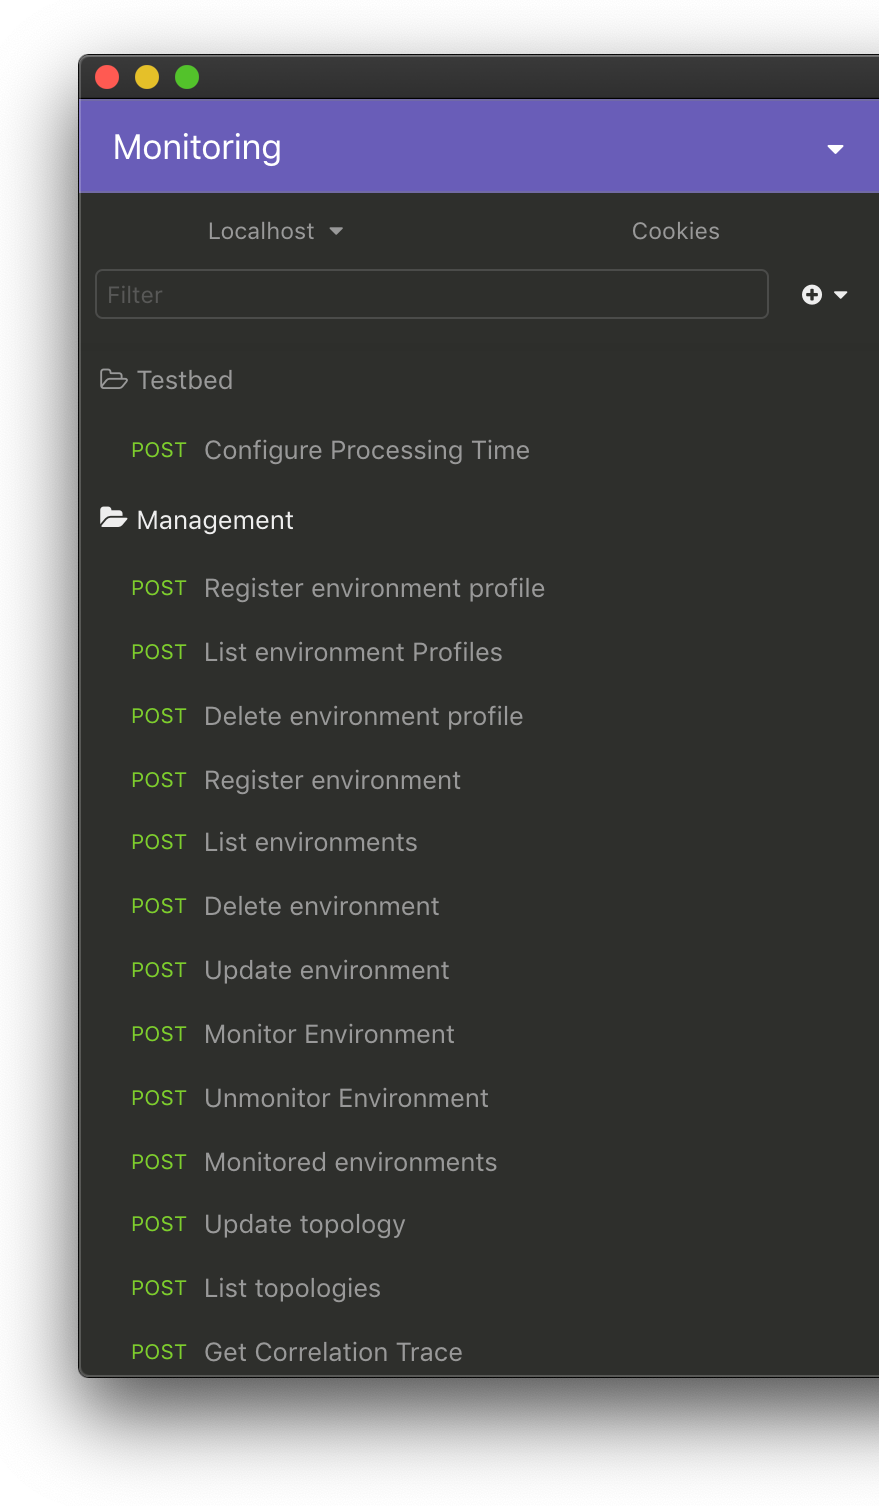
\includegraphics[scale=0.4]{figures/walkthrough/graphql_operations.png}
	\caption{GraphQL interface - All supported operations.}
	\label{walkthough_graphql_operations}
\end{figure}

\section{Kafka Environment Monitoring with the Kubernetes Discovery Agent}

\begin{enumerate}
	\item Before configuring an environment for monitoring, an environment profile must be created. In Figure \ref{walkthrough_no_profiles}, the currently defined set of environment profiles is queried at the GraphQL client. An empty list is returned by the Management Service. \linebreak

	In Figure \ref{walkthrough_create_profile}, an environment profile named \textbf{KAFKA} is created. This profile defines the monitoring task implementation applied for environments using this profile, \texttt{org.cit.mcaleerj.thesis.monitorservice.task.impl.KafkaMonitoringTask}. As the name of this Java class suggests, the task implementation monitors activity in Kafka-based applications. For an application based on RabbitMQ or ActiveMQ, an alternate classname would be specified here.

 \begin{figure}[H]
	\centering  
	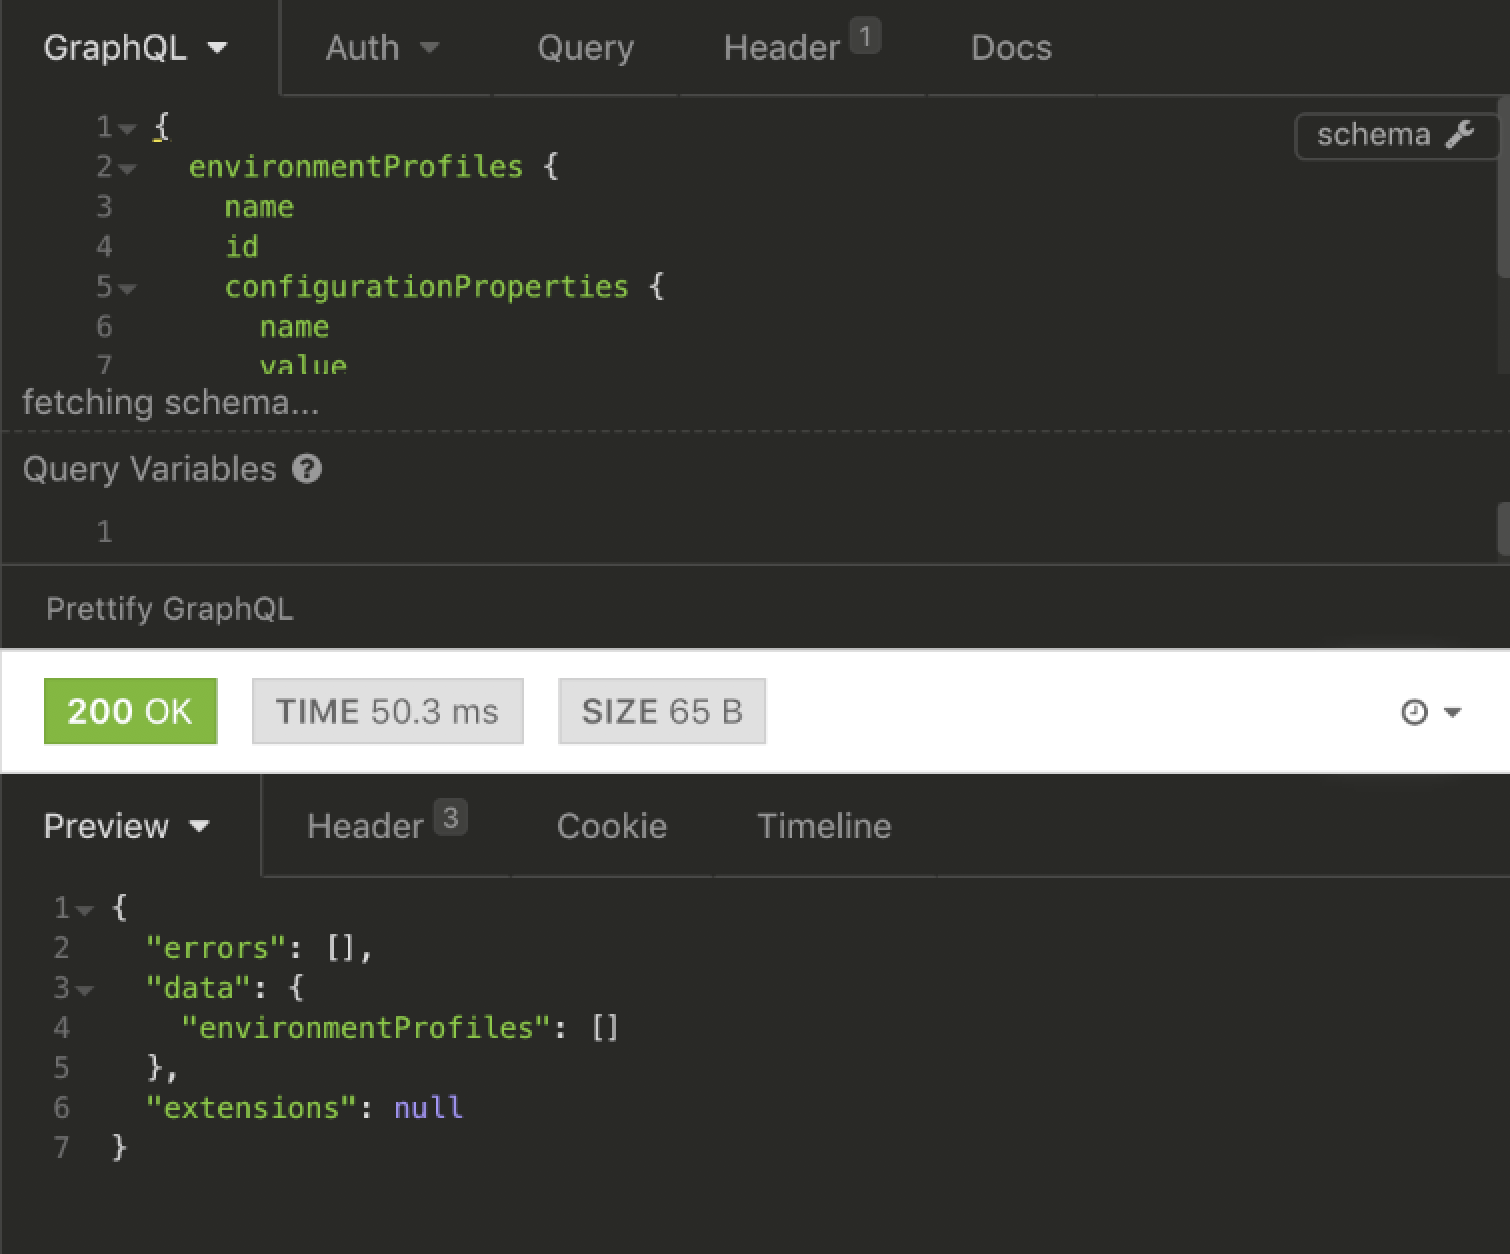
\includegraphics[scale=0.9]{figures/walkthrough/no-env-profiles.png}
	\caption{GraphQL interface - No environment profiles defined.}
	\label{walkthrough_no_profiles}
\end{figure}

 \begin{figure}[H]
	\centering  
	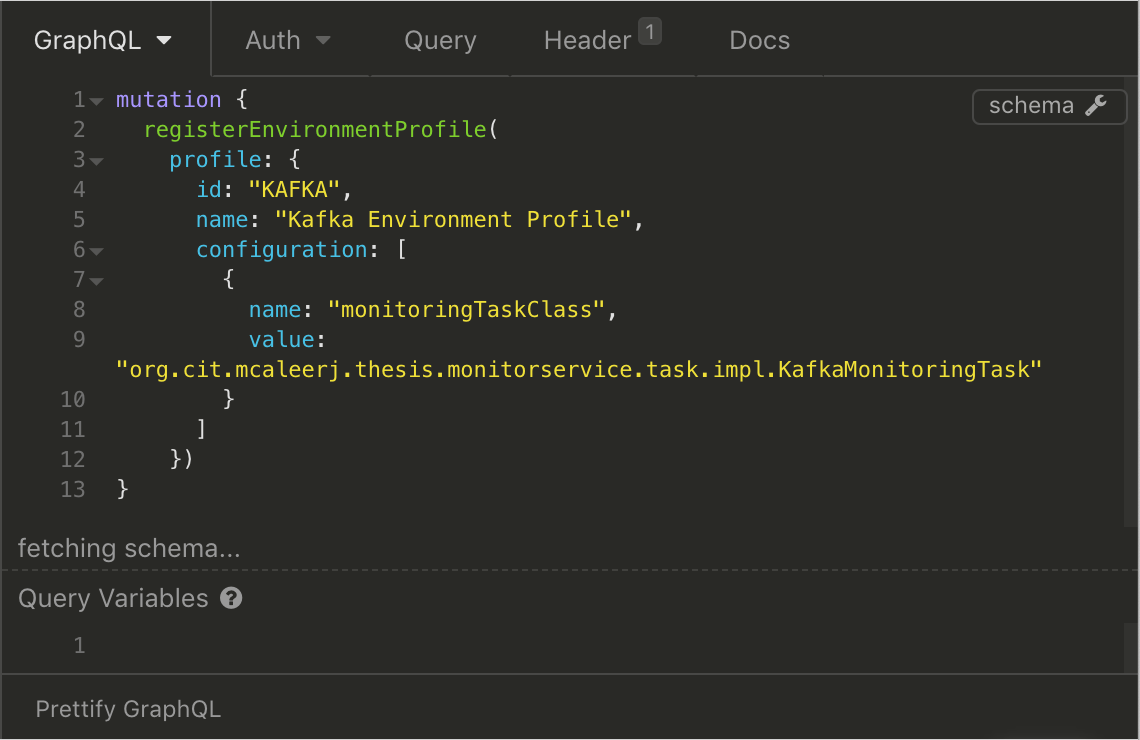
\includegraphics[scale=0.6]{figures/walkthrough/register_env_profile.png}
	\caption{GraphQL interface - KAFKA environment profile created.}
	\label{walkthrough_create_profile}
\end{figure}

	\item  In this step, an environment is defined with the following attributes:
	\begin{itemize}
		\item The environment is named \textbf{Test Environment}
		\item The environment uses the \textbf{KAFKA} profile.
		\item Configuration property \texttt{bootstrap-servers} is set to the address of the monitored application's Kafka broker: \texttt{bootstrap.kafka:9092}.
		\item Configuration property \texttt{discovery.agent.k8s.cert.path} is set to the address of a client certificate for the test bed Kubernetes cluster. This property will be read by the Kubernetes Discovery Agent.
		\item Configuration property \texttt{discovery.agent.k8s.namespace} is set to the name of the Kubernetes namespace in which the testbed pipeline will run. This property will be read by the Kubernetes Discovery Agent.
		
		 \vspace{5mm}
		 
		Figure \ref{walkthrough_env_creation} demonstrates registration of an environment using the GraphQL interface. In Figure \ref{walkthrough_env_list}, a query for the current set of registered environments returns the newly-registered environment definition. Note that a UUID is automatically generated for and assigned to newly registered environments.
		 \vspace{5mm}
  \end{itemize}
 \begin{figure}[H]
	\centering  
	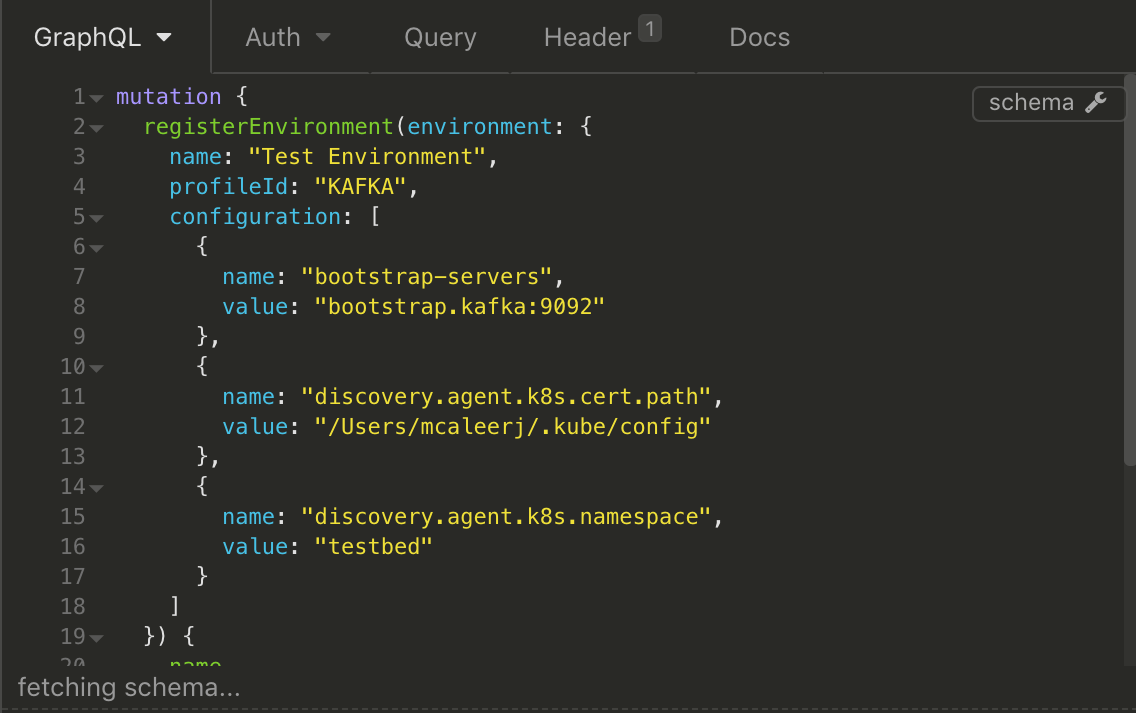
\includegraphics[scale=0.6]{figures/walkthrough/register_env.png}
	\caption{GraphQL interface - Registration of the test bed environment.}
	\label{walkthrough_env_creation}
\end{figure}

 \begin{figure}[H]
	\centering  
	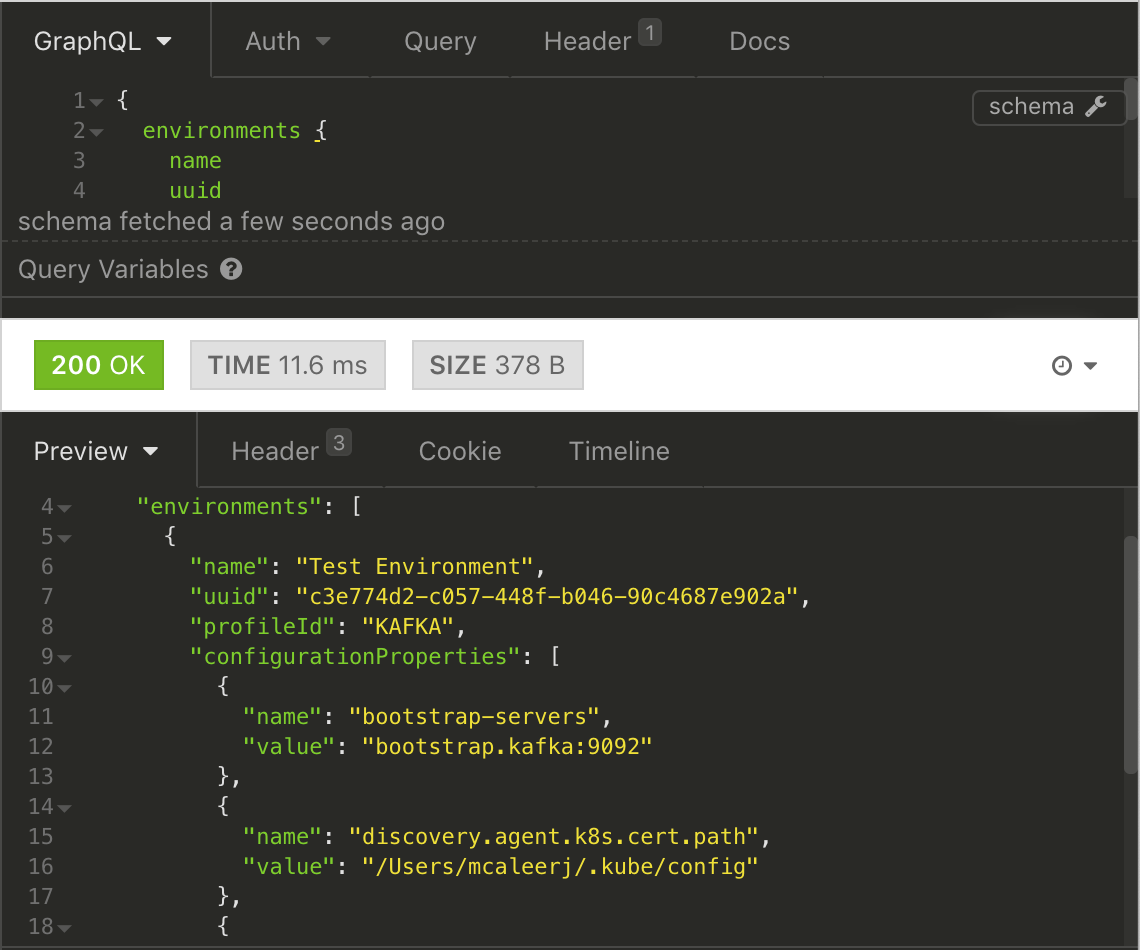
\includegraphics[scale=0.6]{figures/walkthrough/list_envs.png}
	\caption{GraphQL interface - test bed environment configuration complete.}
	\label{walkthrough_env_list}
\end{figure}

\item  In Figure \ref {walkthough_list_topologies_empty}, a query for the current set of known topologies is executed against the Management Service GraphQL endpoint. The Management Service returns an empty list. While a single environment has been registered, monitoring has not yet been enabled for the environment, and thus no discovery agents or monitoring tasks are executing against the environment as of yet.

 \begin{figure}[H]
	\centering  
	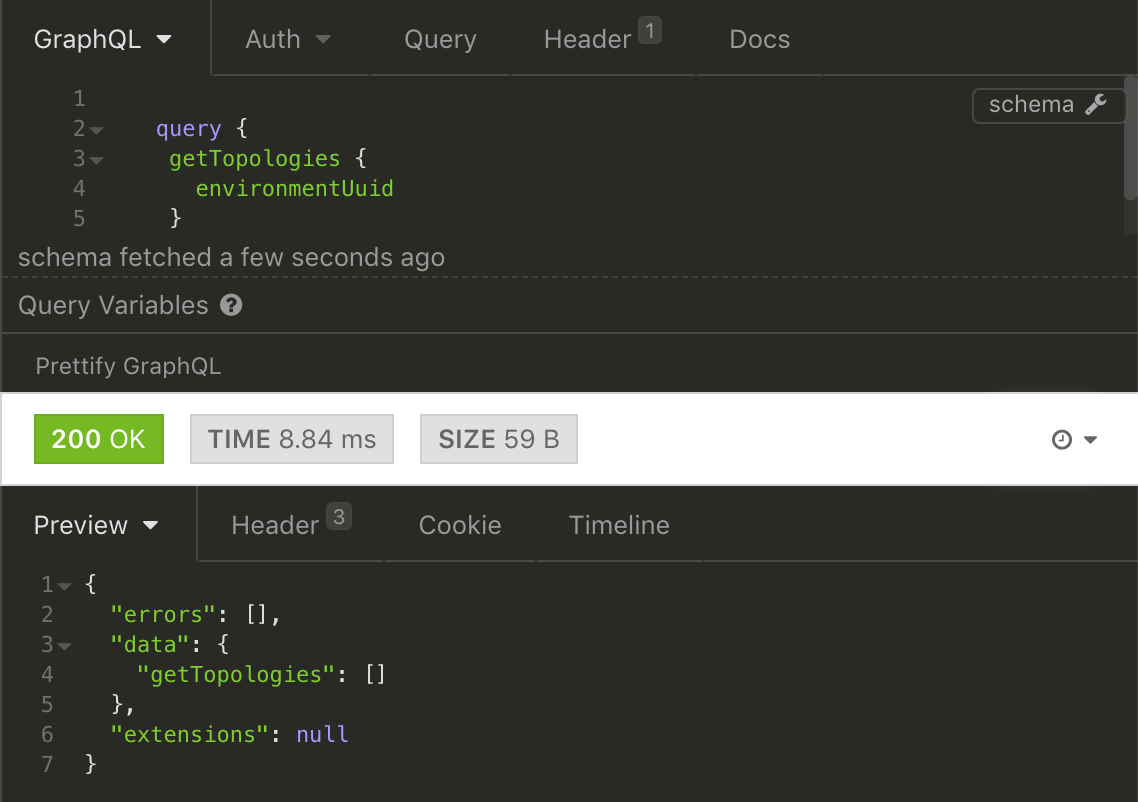
\includegraphics[scale=0.6]{figures/walkthrough/no_topologies.png}
	\caption{GraphQL interface -  No topologies defined.}
	\label{walkthough_list_topologies_empty}
\end{figure}

\item  Using the generated UUID for the environment registered in previous steps, environment monitoring is enabled in Figure \ref{walkthough_enabled_monitoring}.

 \begin{figure}[H]
	\centering  
	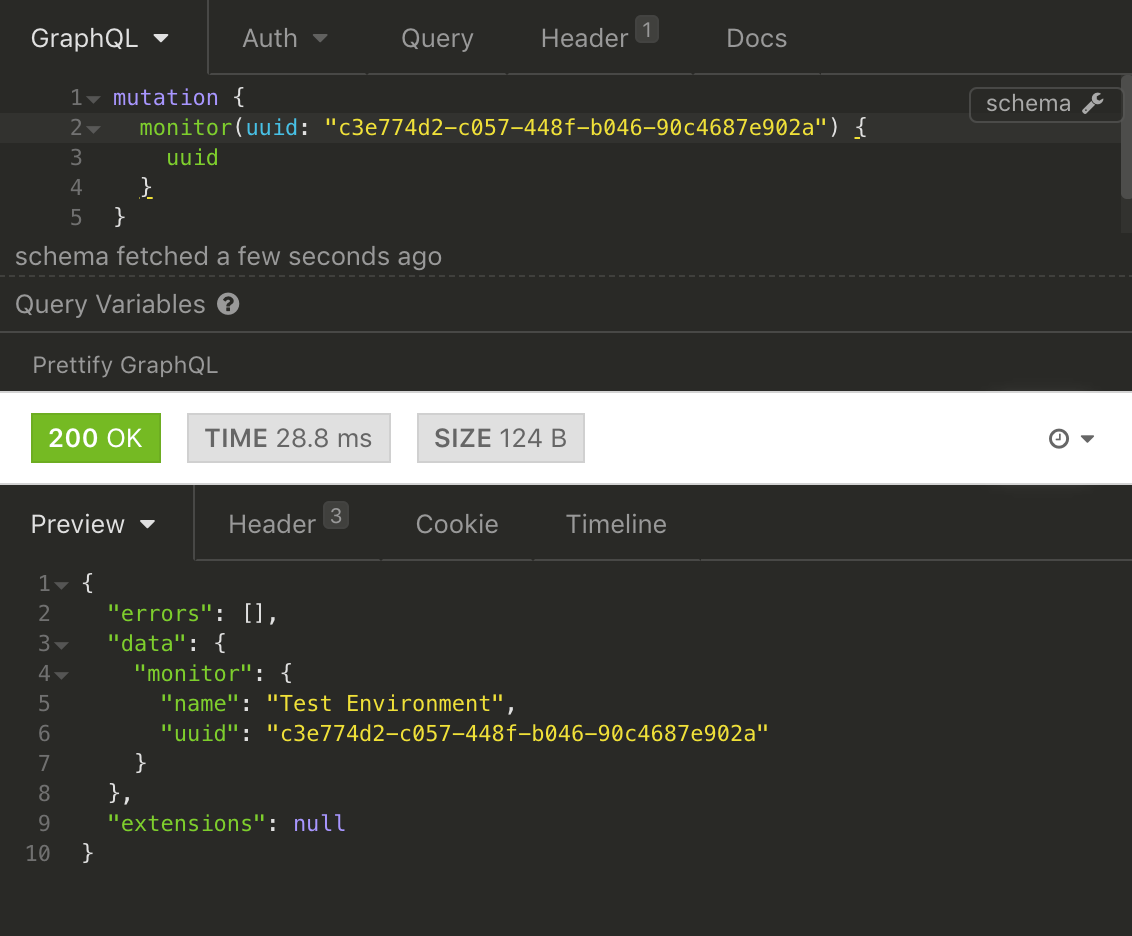
\includegraphics[scale=0.6]{figures/walkthrough/enable_monitoring.png}
	\caption{GraphQL interface -  Enabling monitoring for the test bed environment.}
	\label{walkthough_enabled_monitoring}
\end{figure}

\item The Dashboard Client is opened for the monitored environment. No topology is displayed, as the test bed application has not yet been deployed. The empty topology rendition is portrayed in Figure \ref{walkthough_empty_topology}.

 \begin{figure}[H]
	\centering  
	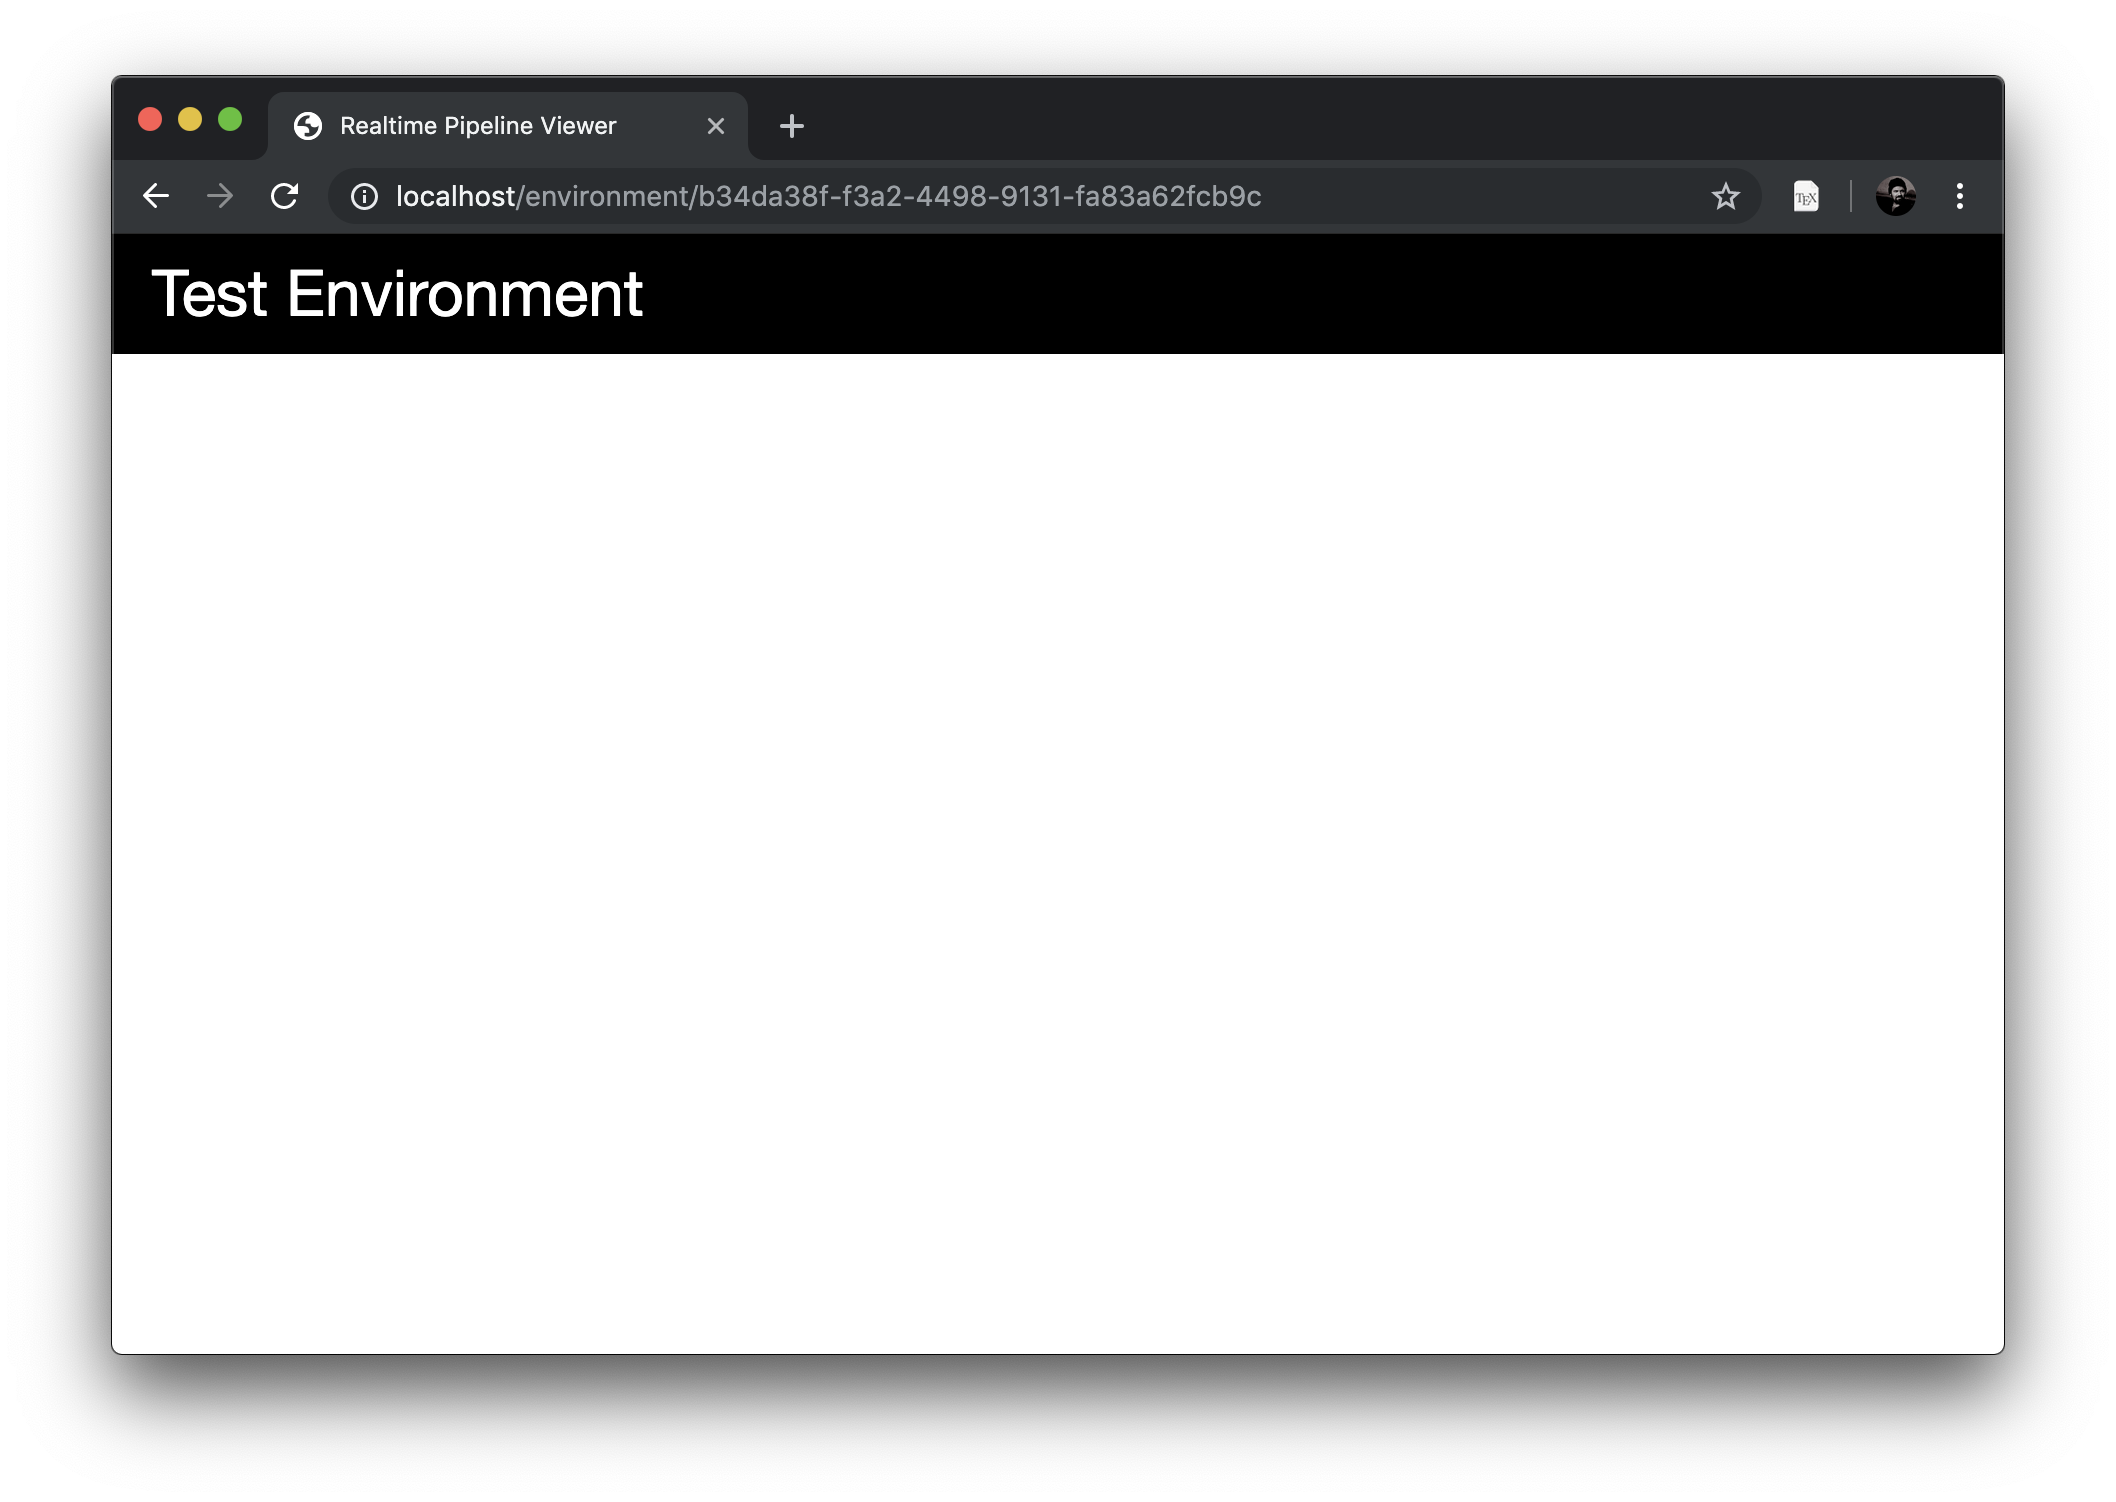
\includegraphics[scale=0.3]{figures/walkthrough/env-zero-nodes.png}
	\caption{Dashboard Client - test bed environment contains an empty topology.}
	\label{walkthough_empty_topology}
\end{figure}

\item Following the steps described in Appendix A, the first of the test bed environment microservices is deployed. The Dashboard Client automatically updates to reflect this change, as depicted in Figure \ref{walkthough_one_node_topology}. The green node indicates an external message source, while the light blue node represents a microservice; the red node meanwhile represents a message sink.

\begin{figure}[H]
	\centering  
	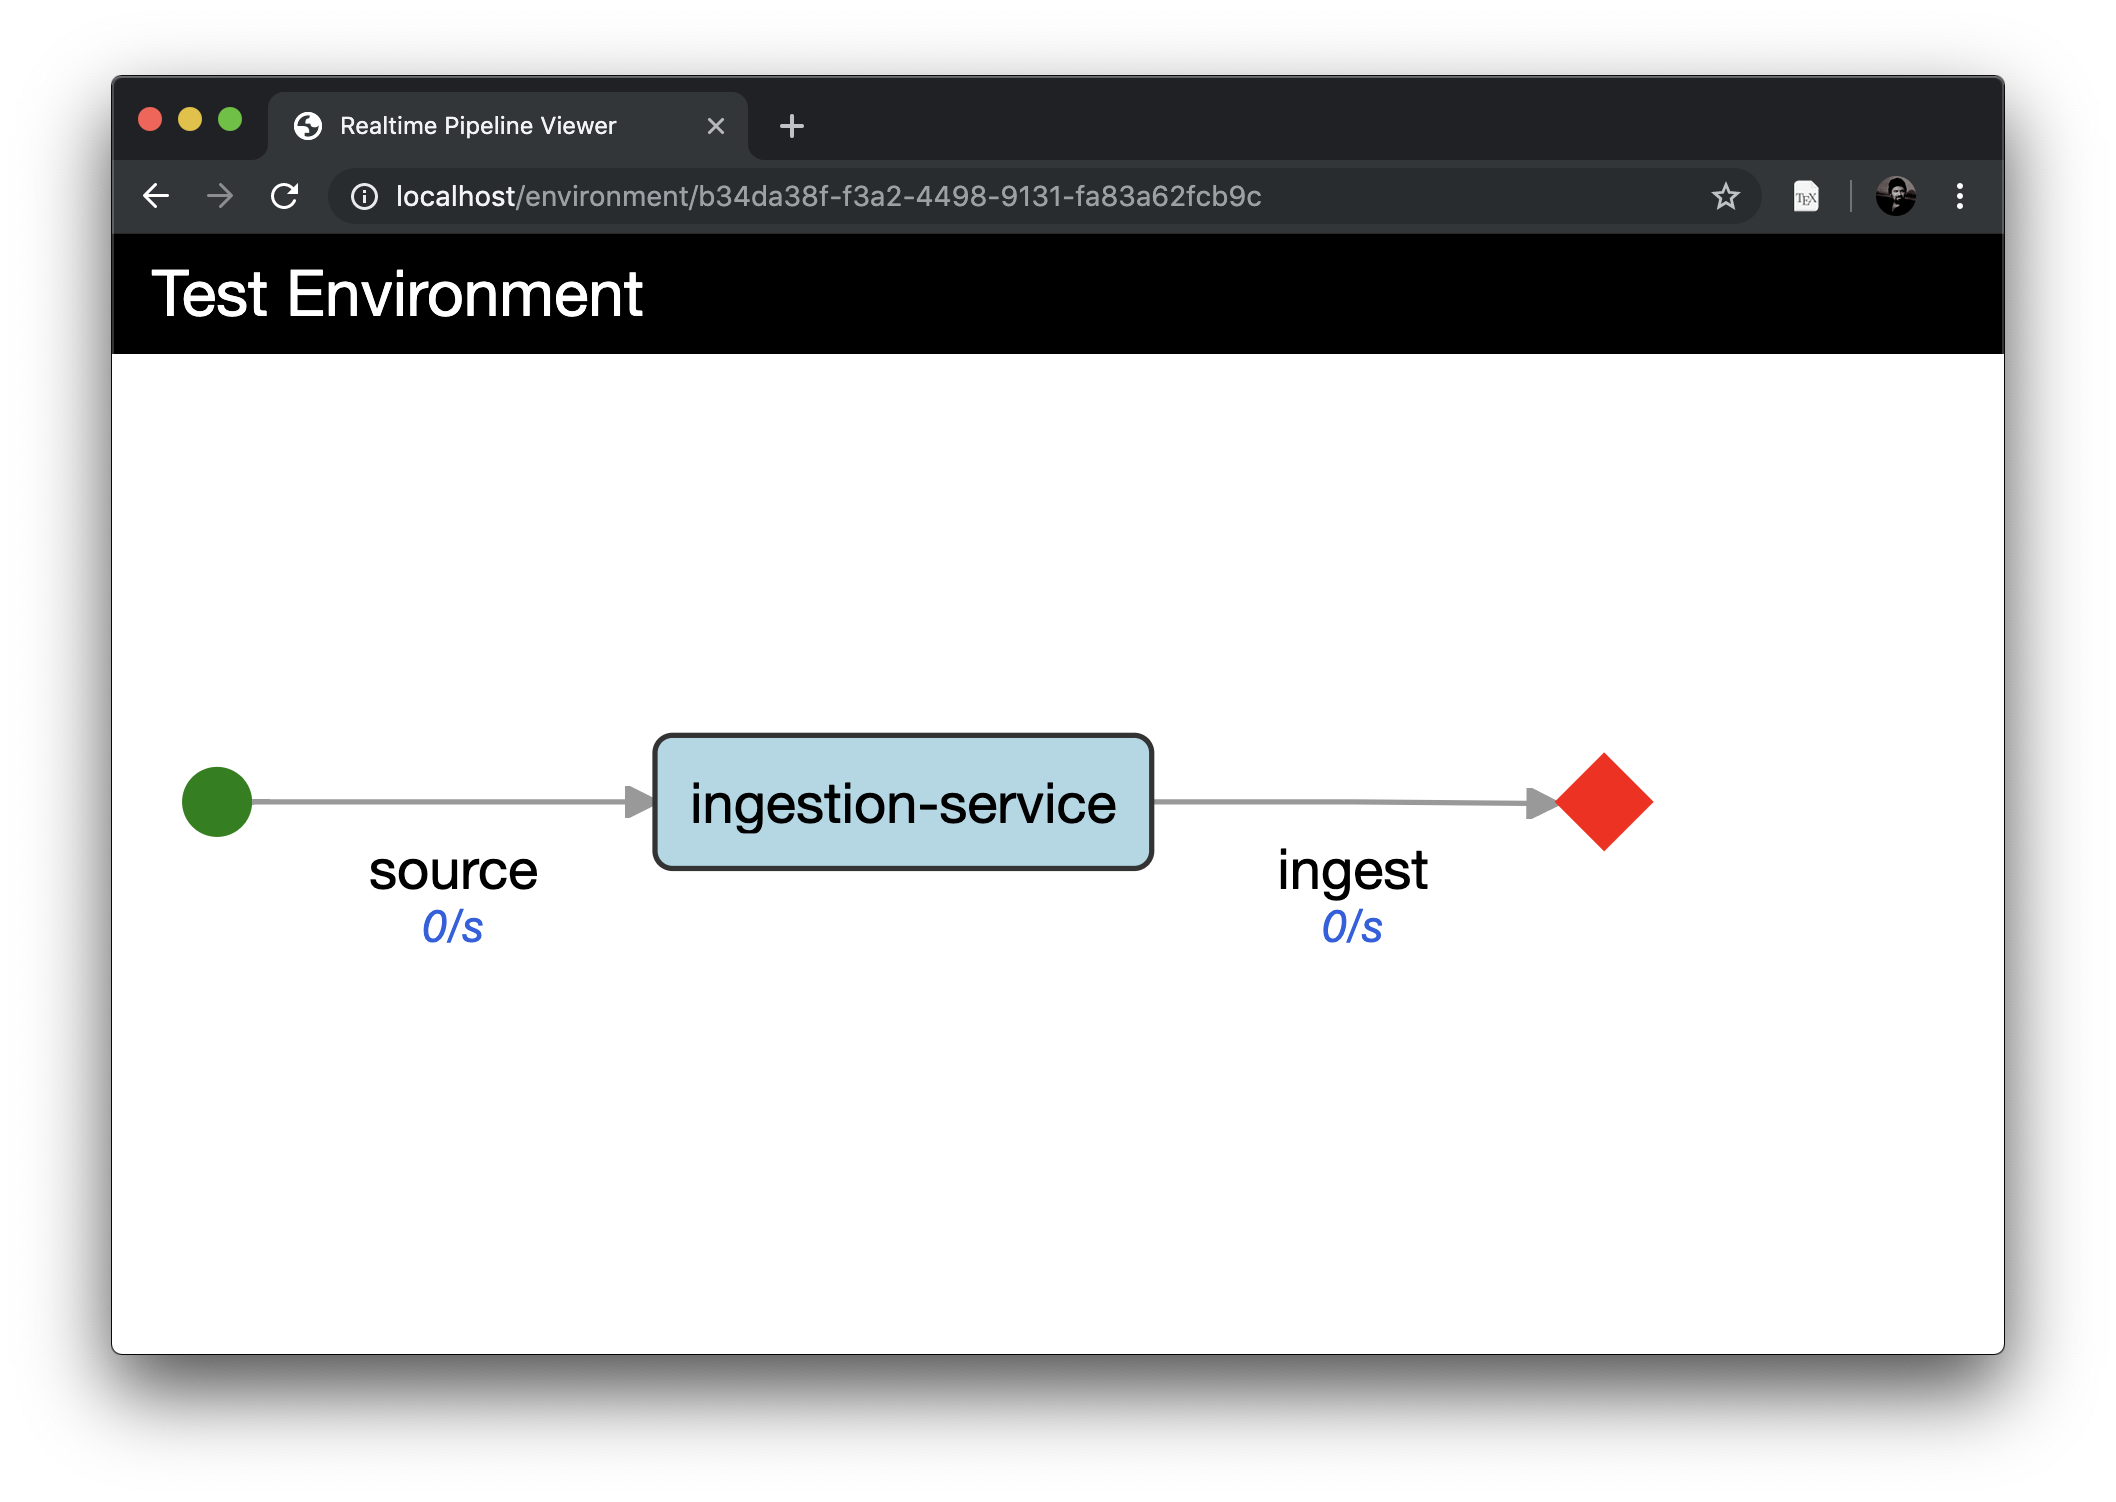
\includegraphics[scale=0.3]{figures/walkthrough/env-one-node.png}
	\caption{Dashboard Client - test bed environment comprising a single microservice.}
	\label{walkthough_one_node_topology}
\end{figure}

\item A second microservice is now deployed; the Dashboard Client again reflects this change automatically, as depicted in Figure \ref{walkthough_two_node_topology}. The ingest edge is no longer rendered as a message sink, as the newly-deployed validation-service is known to consume from same. Two new sink edge are added, namely the \texttt{validated} and \texttt{deadletter} edges.

\begin{figure}[H]
	\centering  
	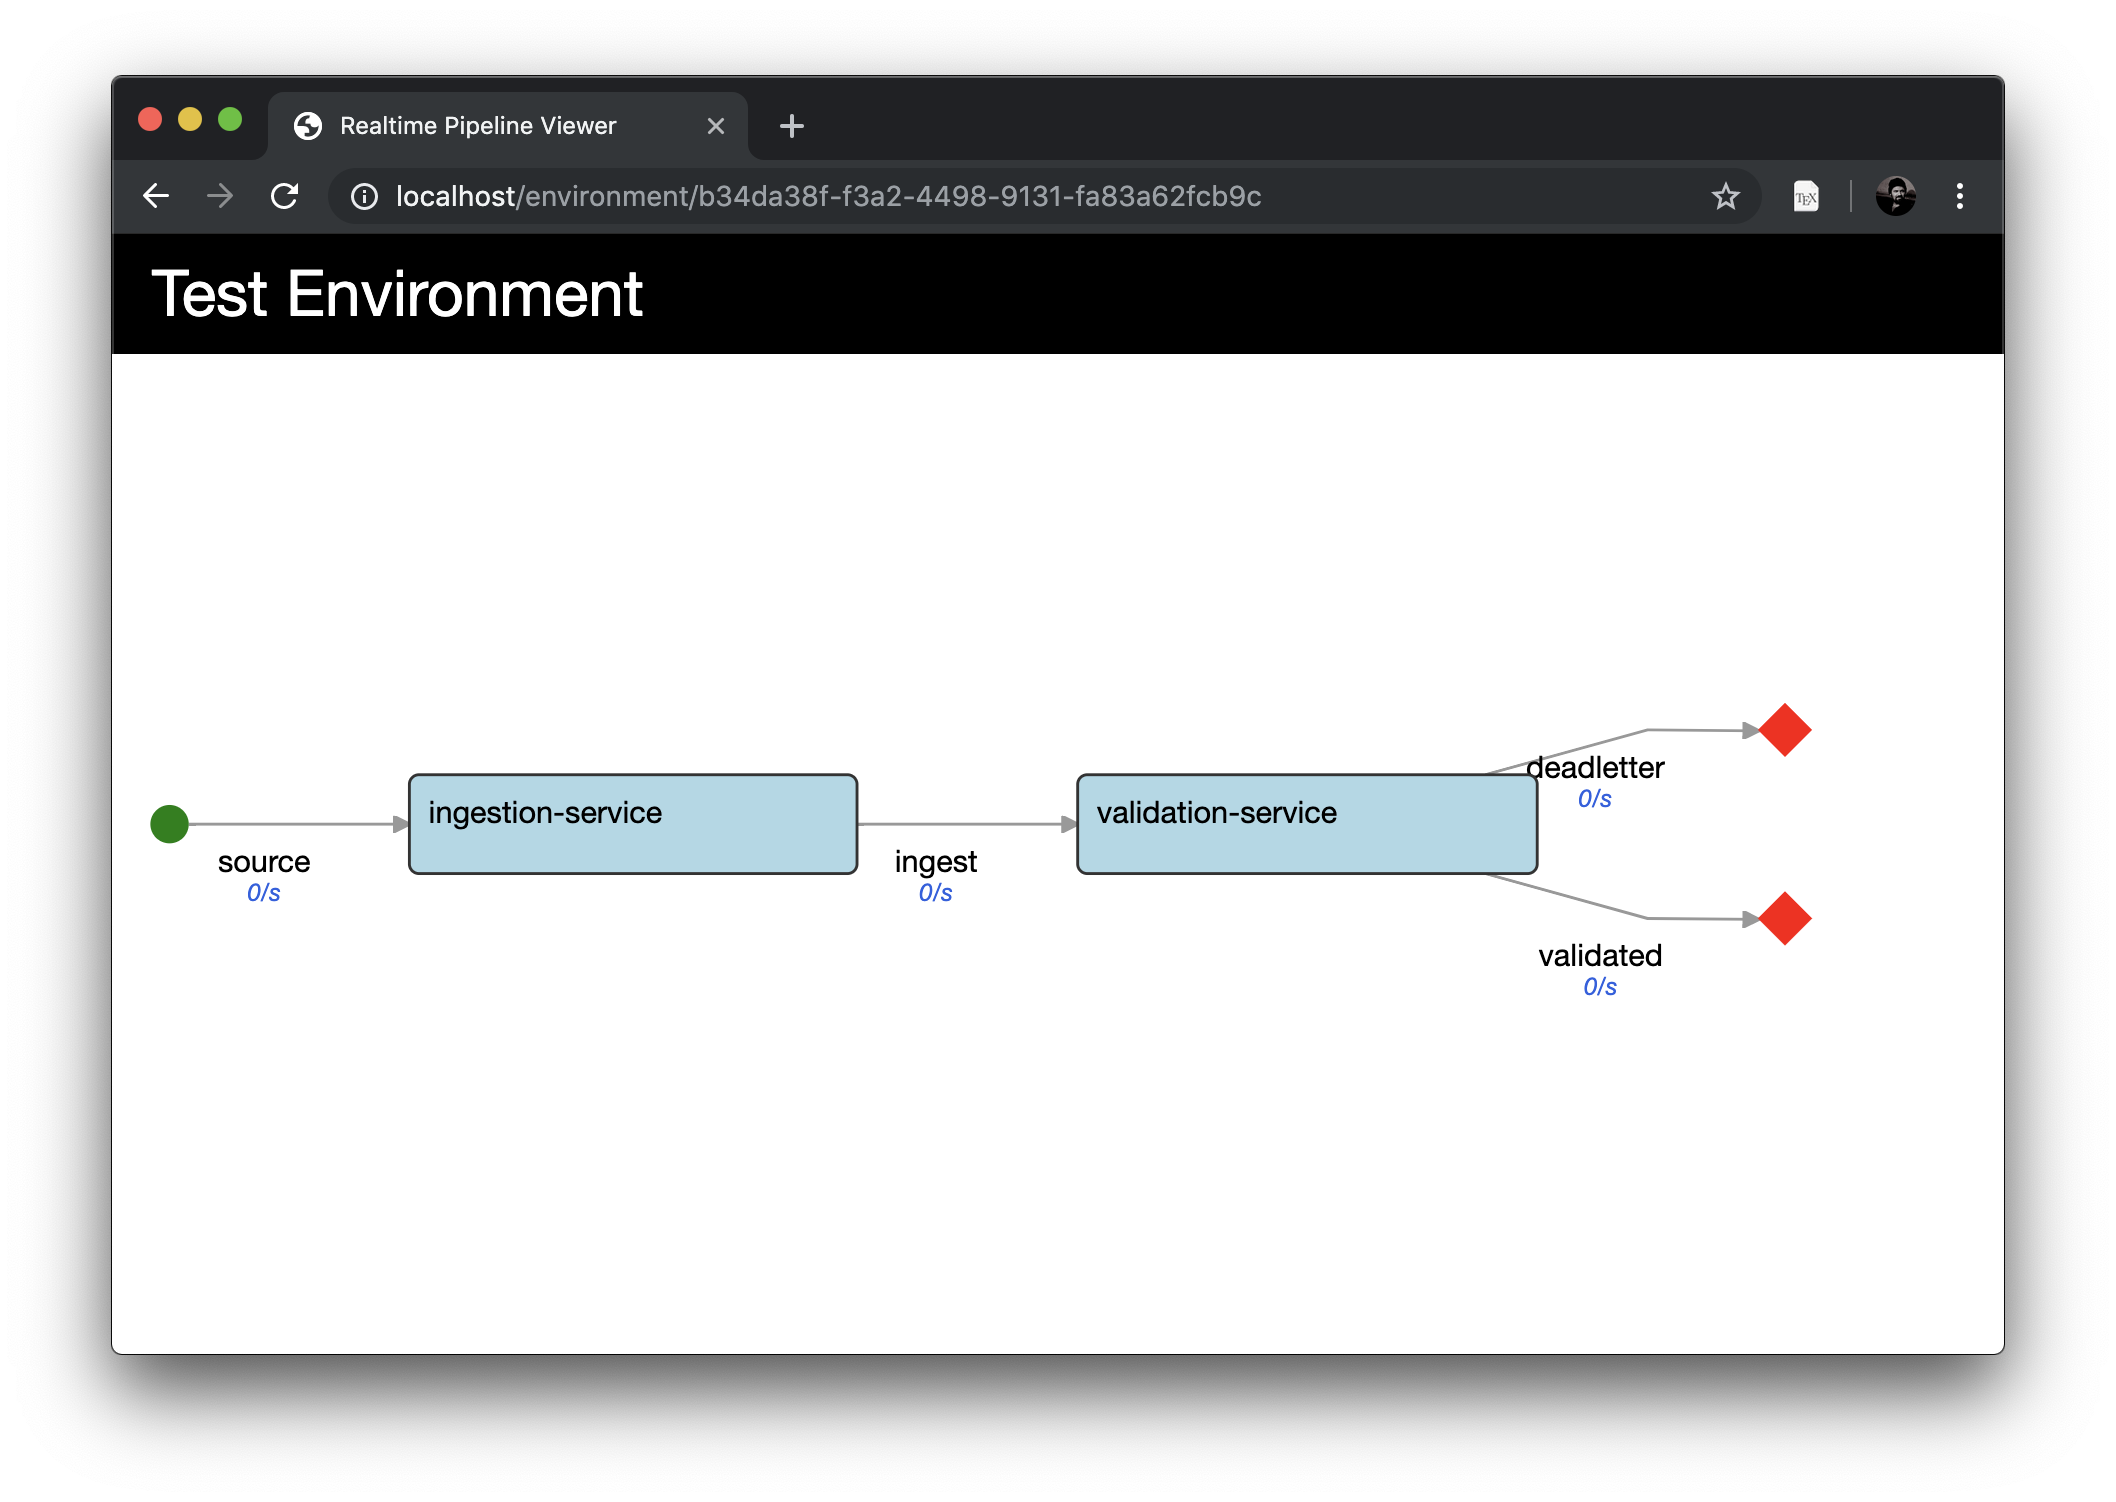
\includegraphics[scale=0.3]{figures/walkthrough/env-two-nodes.png}
	\caption{Dashboard Client - test bed environment comprising two microservices.}
	\label{walkthough_two_node_topology}
\end{figure}

\item The third and final microservice is now deployed; the Dashboard Client again reflects this change automatically, as depicted in Figure \ref{walkthough_three_node_topology}. The validated edge is no longer rendered as a message sink, as the newly-deployed sink-service is known to consume from same. One new sink edge is added, namely the \texttt{processed} edge.

\begin{figure}[H]
	\centering  
	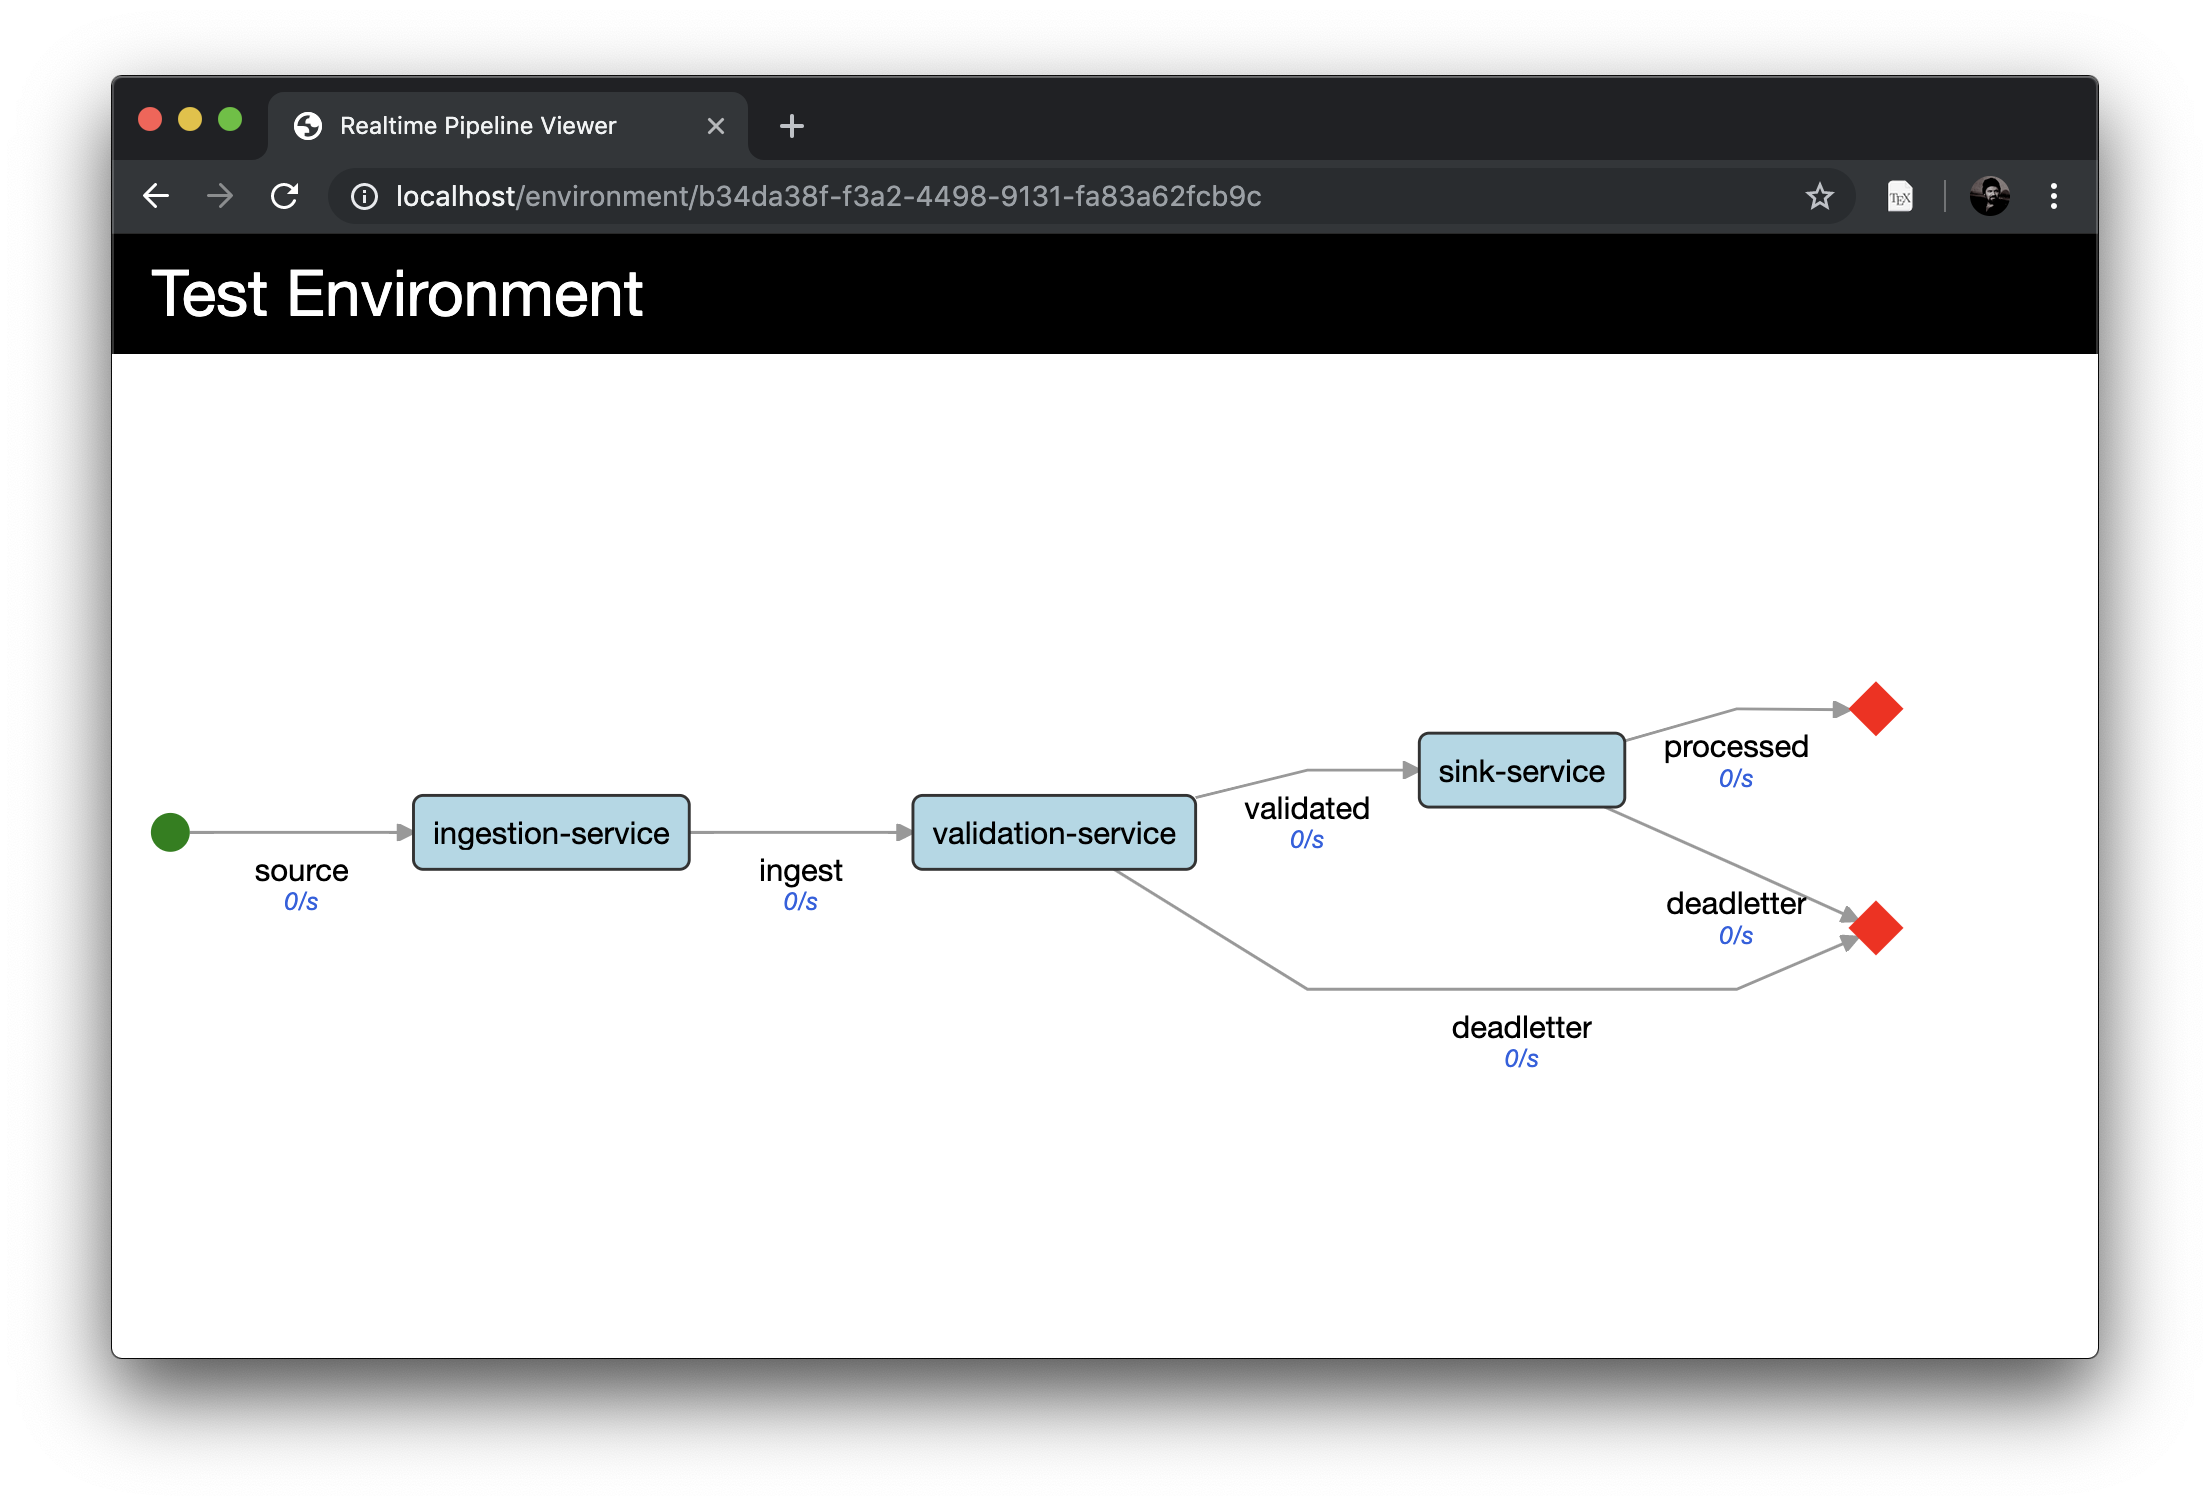
\includegraphics[scale=0.3]{figures/walkthrough/env-three-nodes.png}
	\caption{Dashboard Client - test bed environment comprising three microservices.}
	\label{walkthough_three_node_topology}
\end{figure}

\item Note that edge labels indicate environment activity of zero messages per seconds on all edges in the topology. A message generator is now executed, pushing approximately thirty messages per second to the monitored environment. Topology activity is accurately reflected in real-time by the Dashboard Client, as depicted in Figure \ref{walkthough_thirty_messages_sec}.

\begin{figure}[H]
	\centering  
	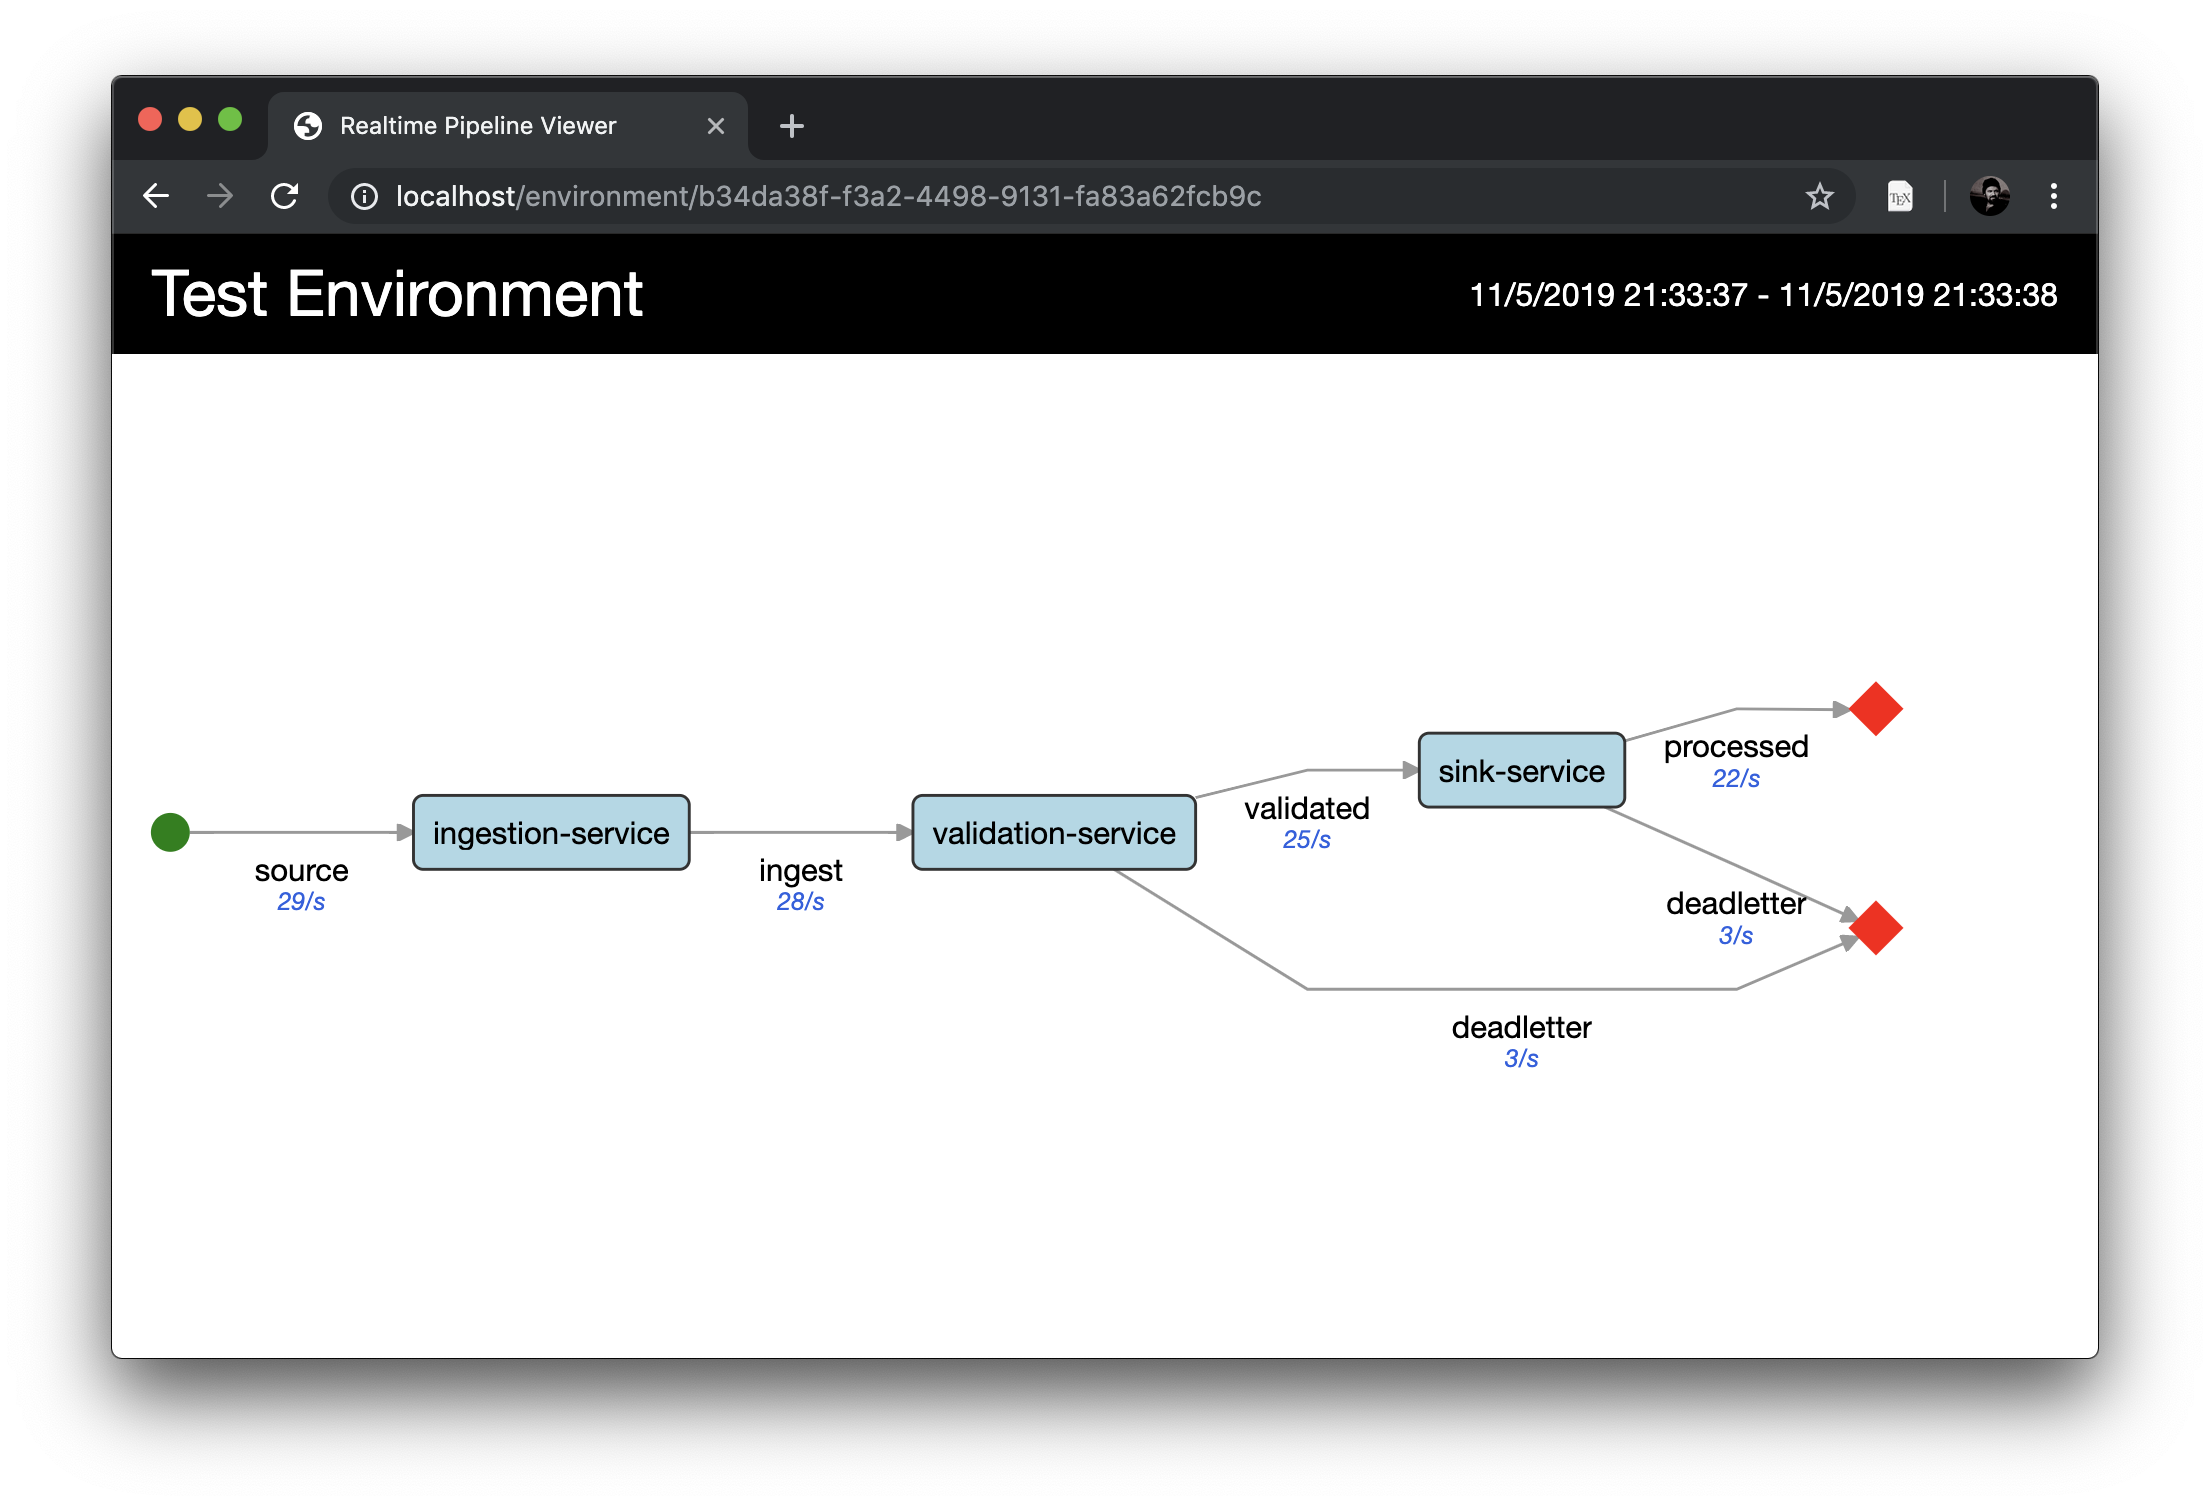
\includegraphics[scale=0.3]{figures/walkthrough/topology_30_sec.png}
	\caption{Dashboard Client - test bed topology processing thirty messages per second.}
	\label{walkthough_thirty_messages_sec}
\end{figure}\

\item The number of messages pushed into the monitored environment is now dropped to approximately ten messages per second. The change in environment throughput is reflected immediately at the Dashboard Client, as depicted in Figure \ref{walkthough_ten_messages_sec}.

\begin{figure}[H]
	\centering  
	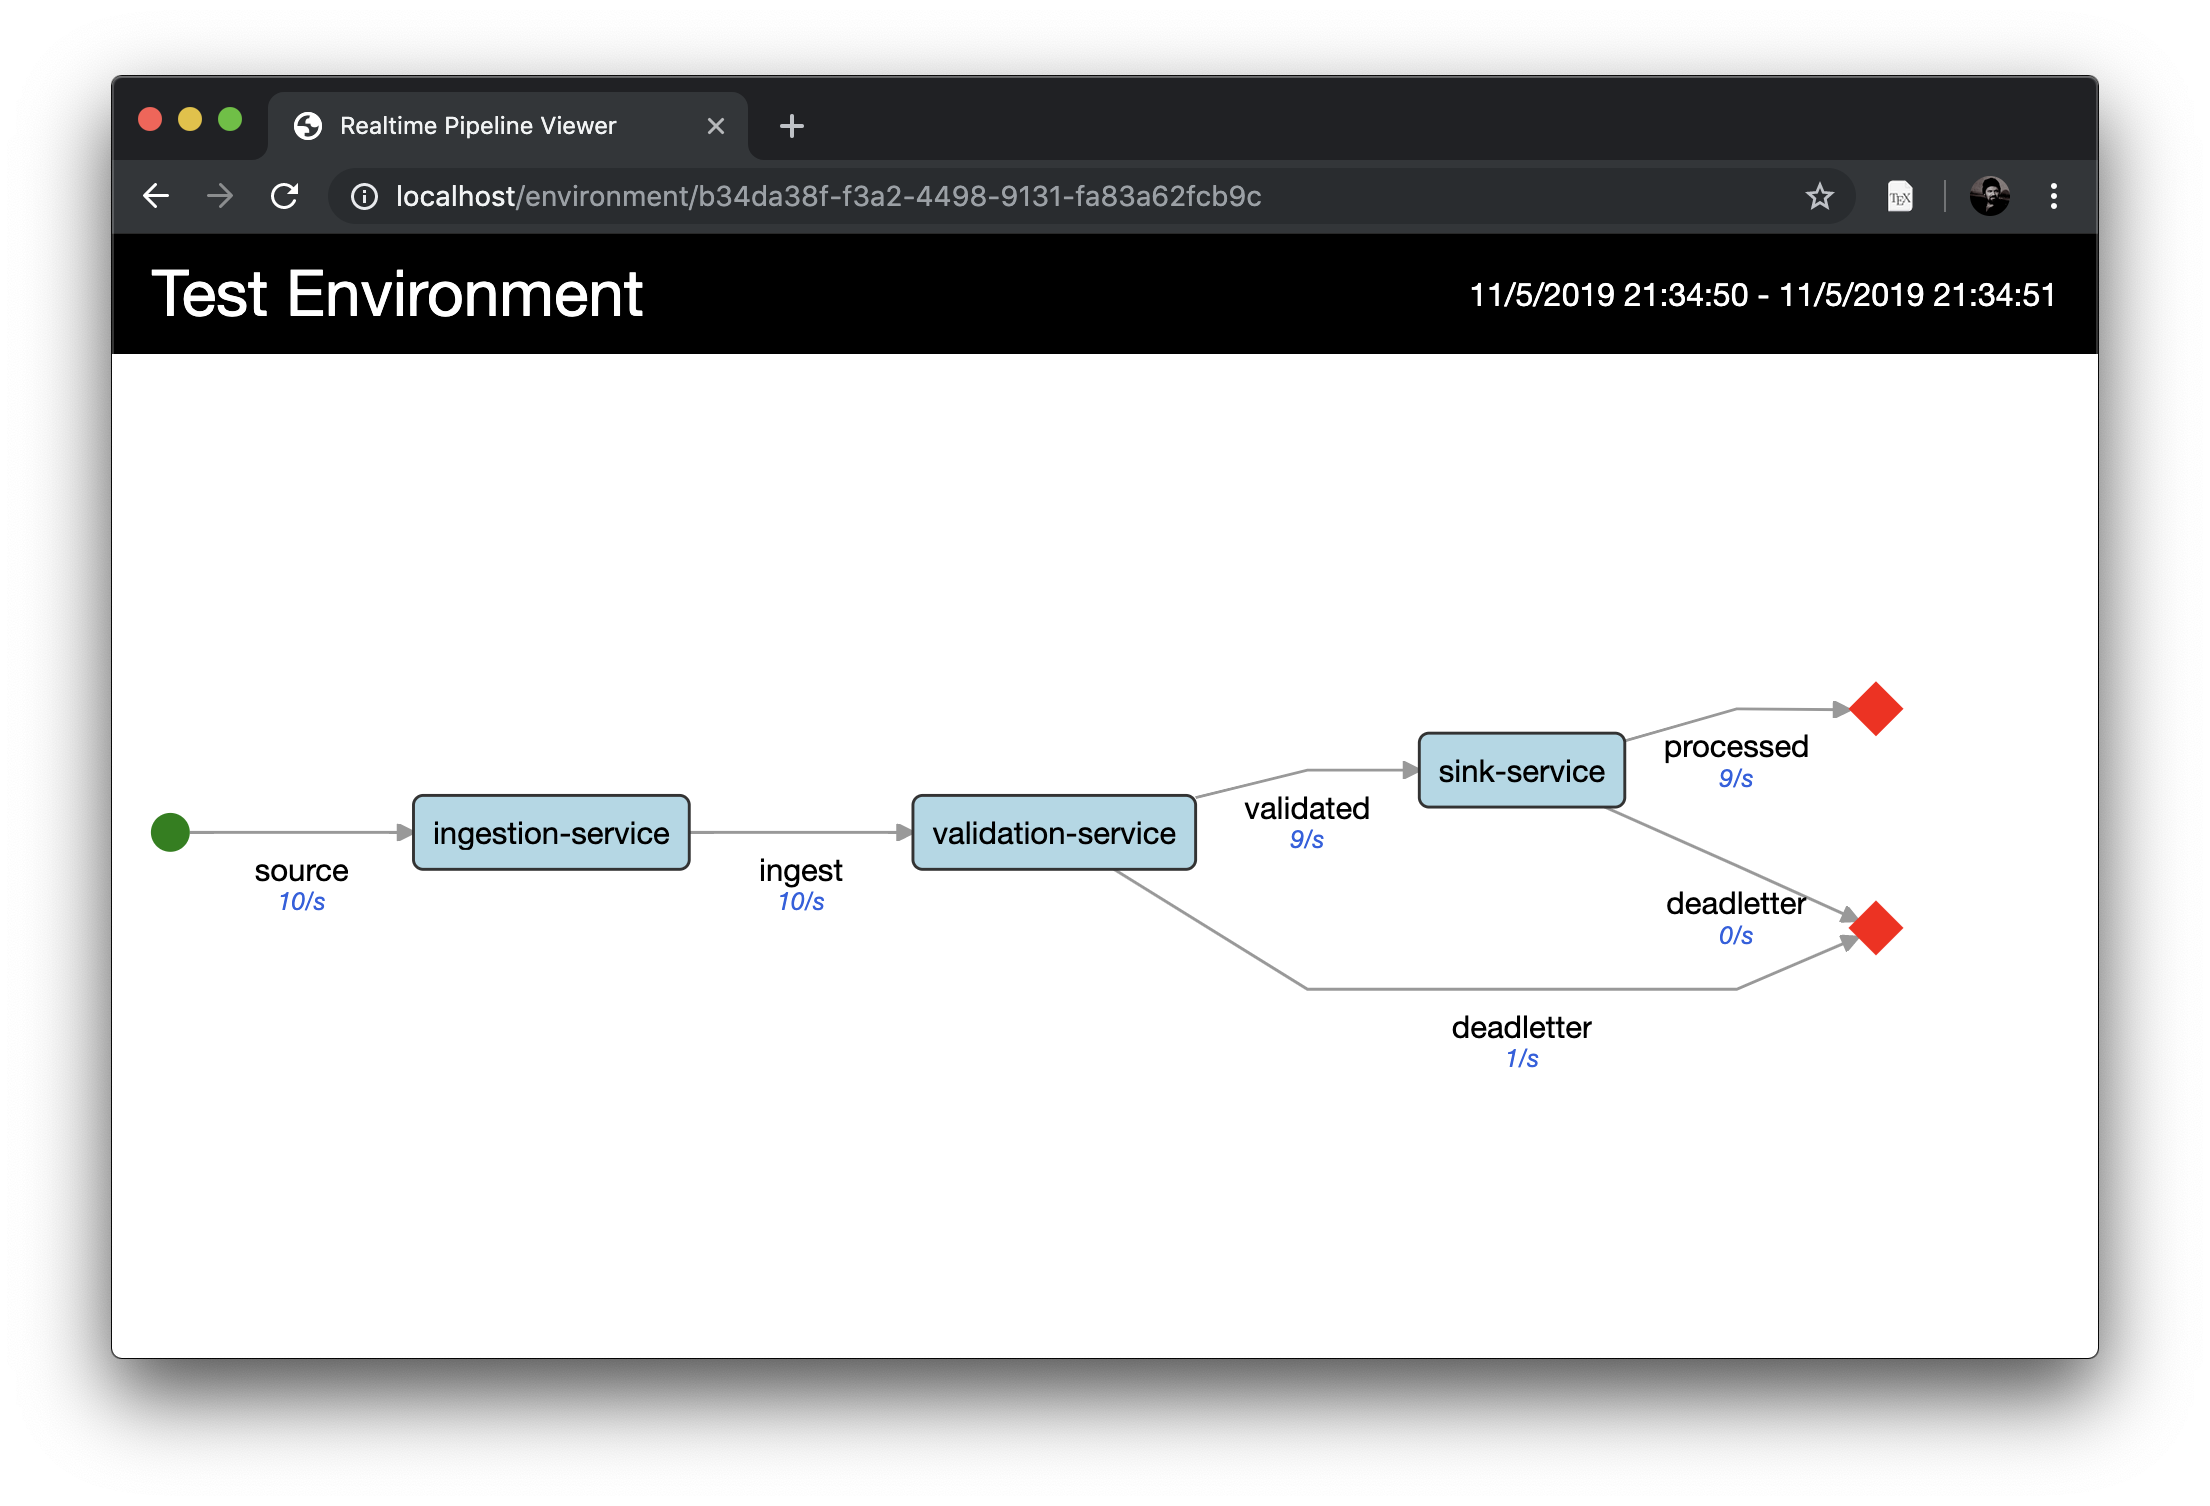
\includegraphics[scale=0.3]{figures/walkthrough/topology_10_sec.png}
	\caption{Dashboard Client - test bed topology processing ten messages per second.}
	\label{walkthough_ten_messages_sec}
\end{figure}

\item The number of messages per second pushed to the environment is restored to thirty per second. An artificial message processing delay is introduced at the validation service, by means of a GraphQL interface provided by same.  The processing bottleneck introduced by this configuration change is clearly reflected by the drop off in throughput on edge \textit{validated}, as demonstrated by Figure \ref{walkthough_bottleneck}.

\begin{figure}[H]
	\centering  
	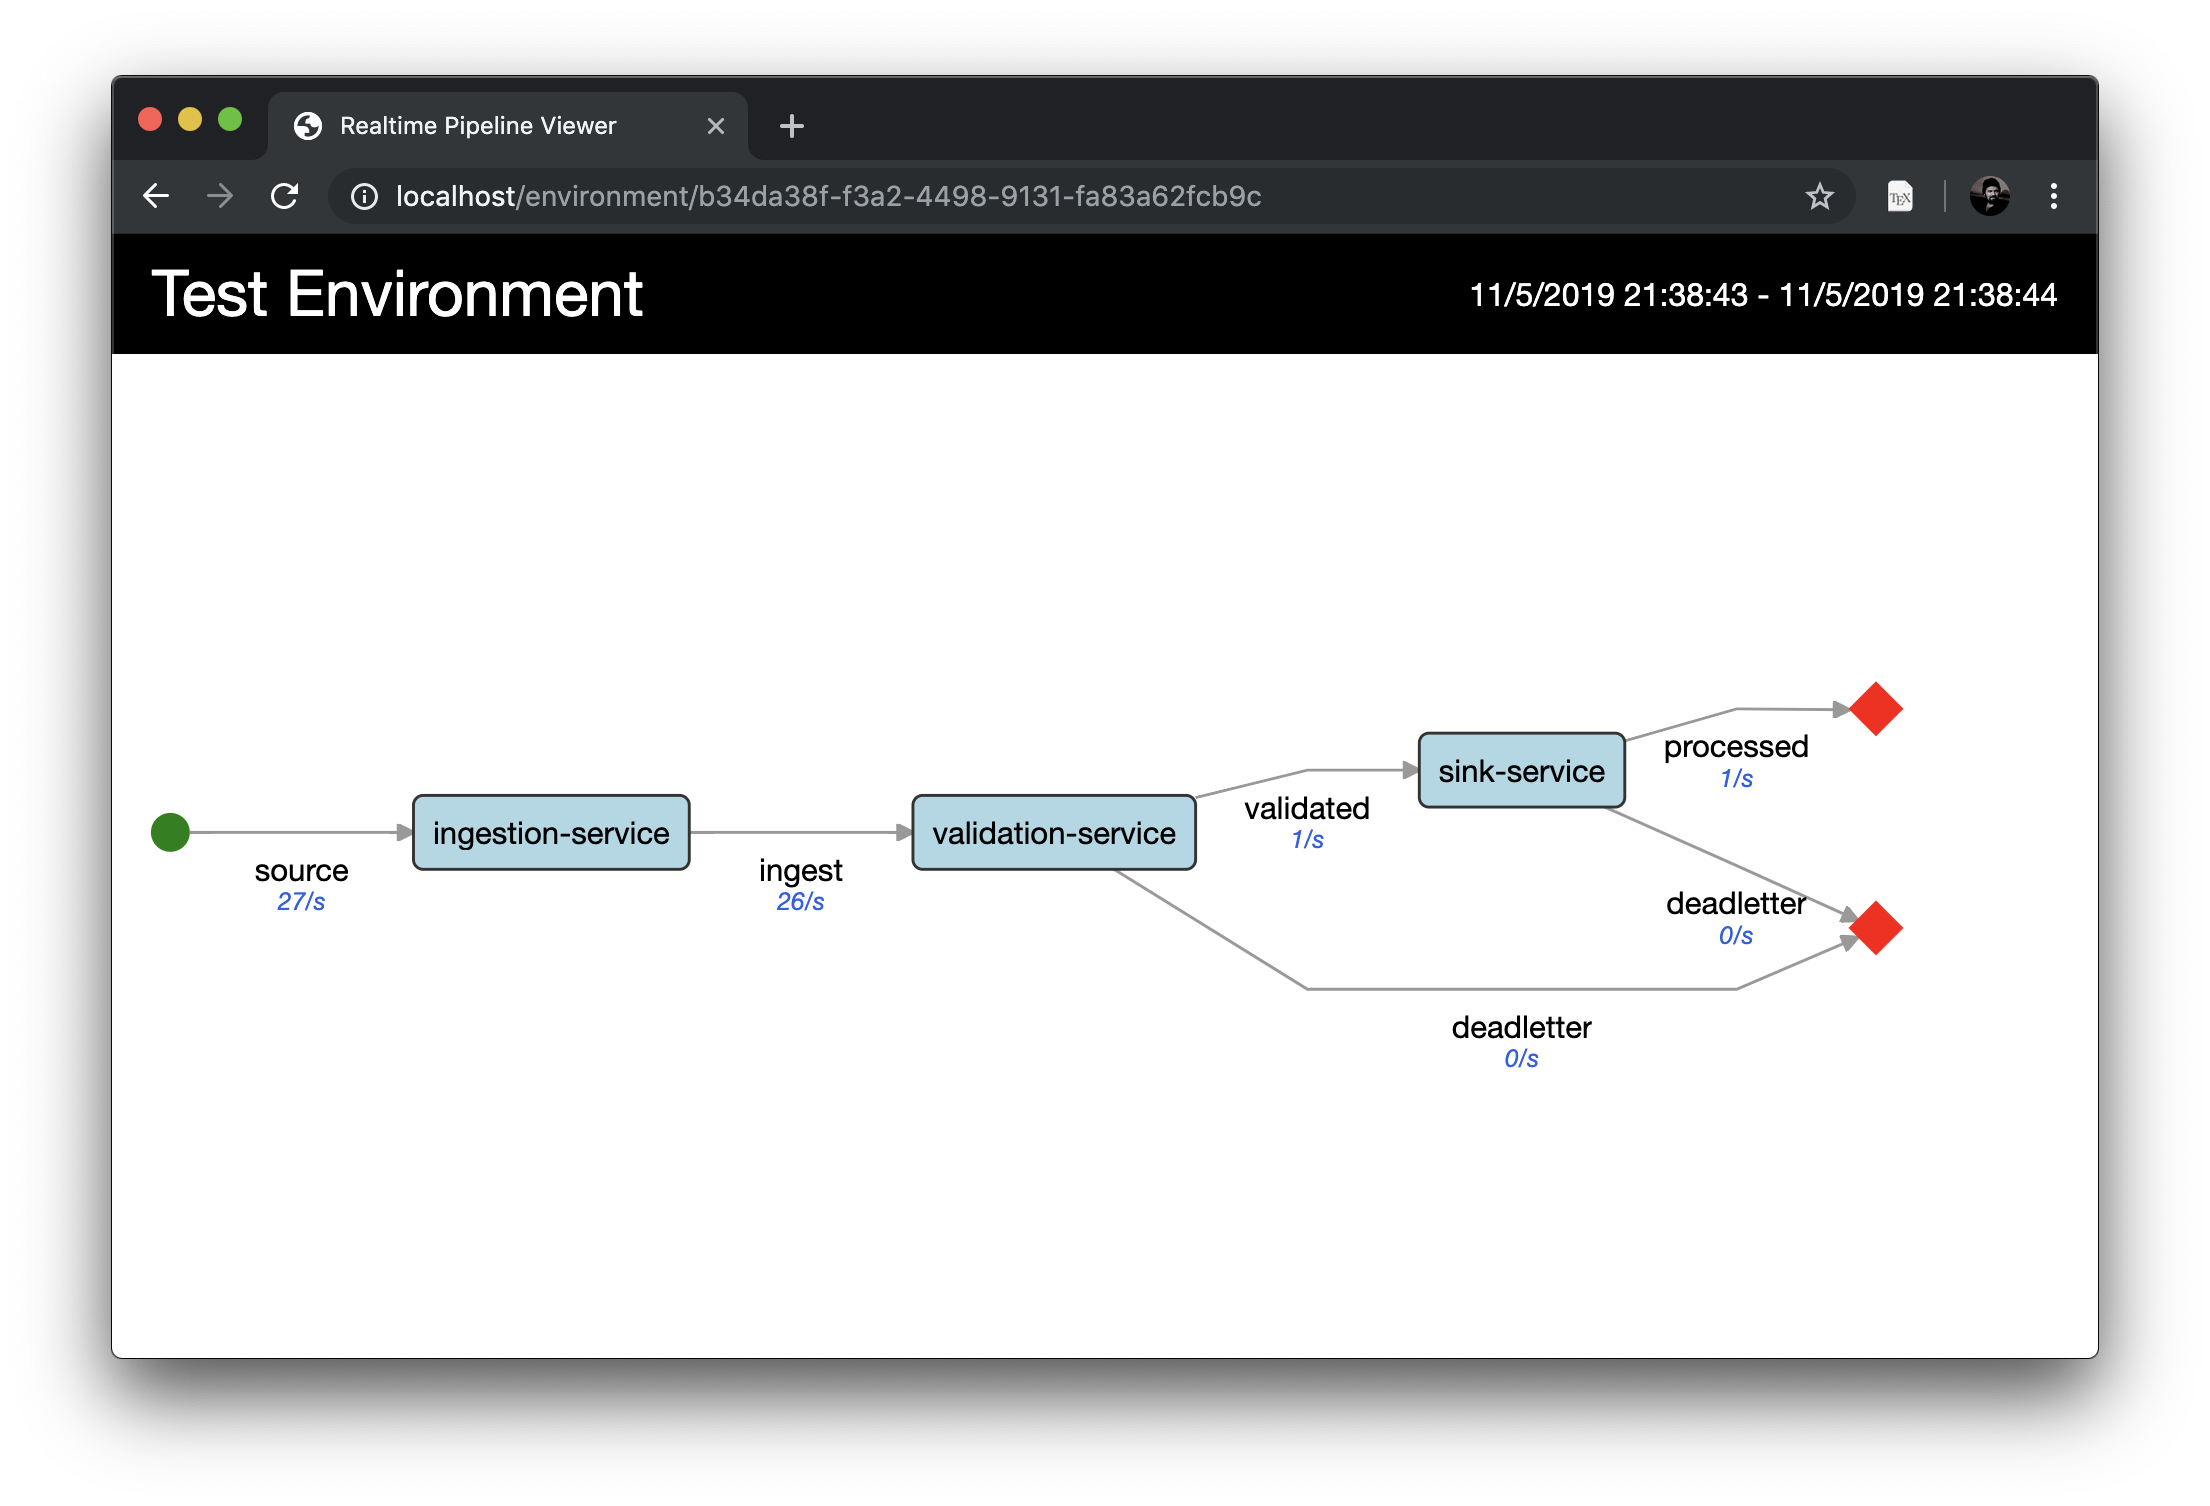
\includegraphics[scale=0.3]{figures/walkthrough/validation_bottleneck.png}
	\caption{Dashboard Client - artificial bottleneck at the validation service.}
	\label{walkthough_bottleneck}
\end{figure}

\end{enumerate}

\section{Environment Monitoring with the Message Correlation Discovery Agent}

\begin{enumerate}
	
	\item A new environment is registered with the monitoring application. For this environment, properties required by the Kubernetes Discovery Agent are not configured. Instead, the Message Correlation Discovery agent is configured by setting environment configuration property \texttt{discovery.agent.correlation.field.name} to \texttt{uuid}. 
	
	Test message payloads sent to the monitored environment each contain a unique UUID field named \texttt{uuid}. The Discovery Agent will leverage this fact, requesting correlation traces based on the configured field from the Correlation Service in order to construct a topology instance. The GraphQL mutation used to configure the newly created environment is depicted in Figure  \ref{reg_env_correlation}.
	
	\vspace{5mm}
		 
\begin{figure}[H]
	\centering  
	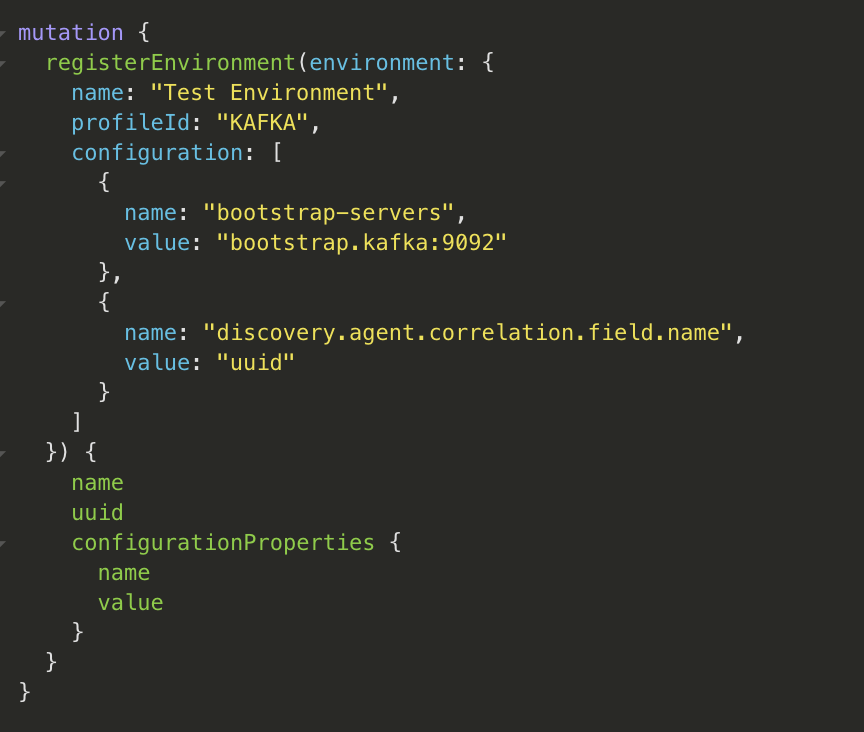
\includegraphics[scale=0.7]{figures/walkthrough/correlation_env.png}
	\caption{Dashboard Client - configuring an environment for correlation-based discovery.}
	\label{reg_env_correlation}
\end{figure}

	\item In contrast to the sequence of events described in the previous section on Kubernetes-based discovery, no topology is rendered until messages begin to flow through the environment. Once a number of messages have traversed the environment, the Dashboard Client renders the topology as depicted in Figure  \ref{activity_env_correlation}.

\begin{figure}[H]
	\centering  
	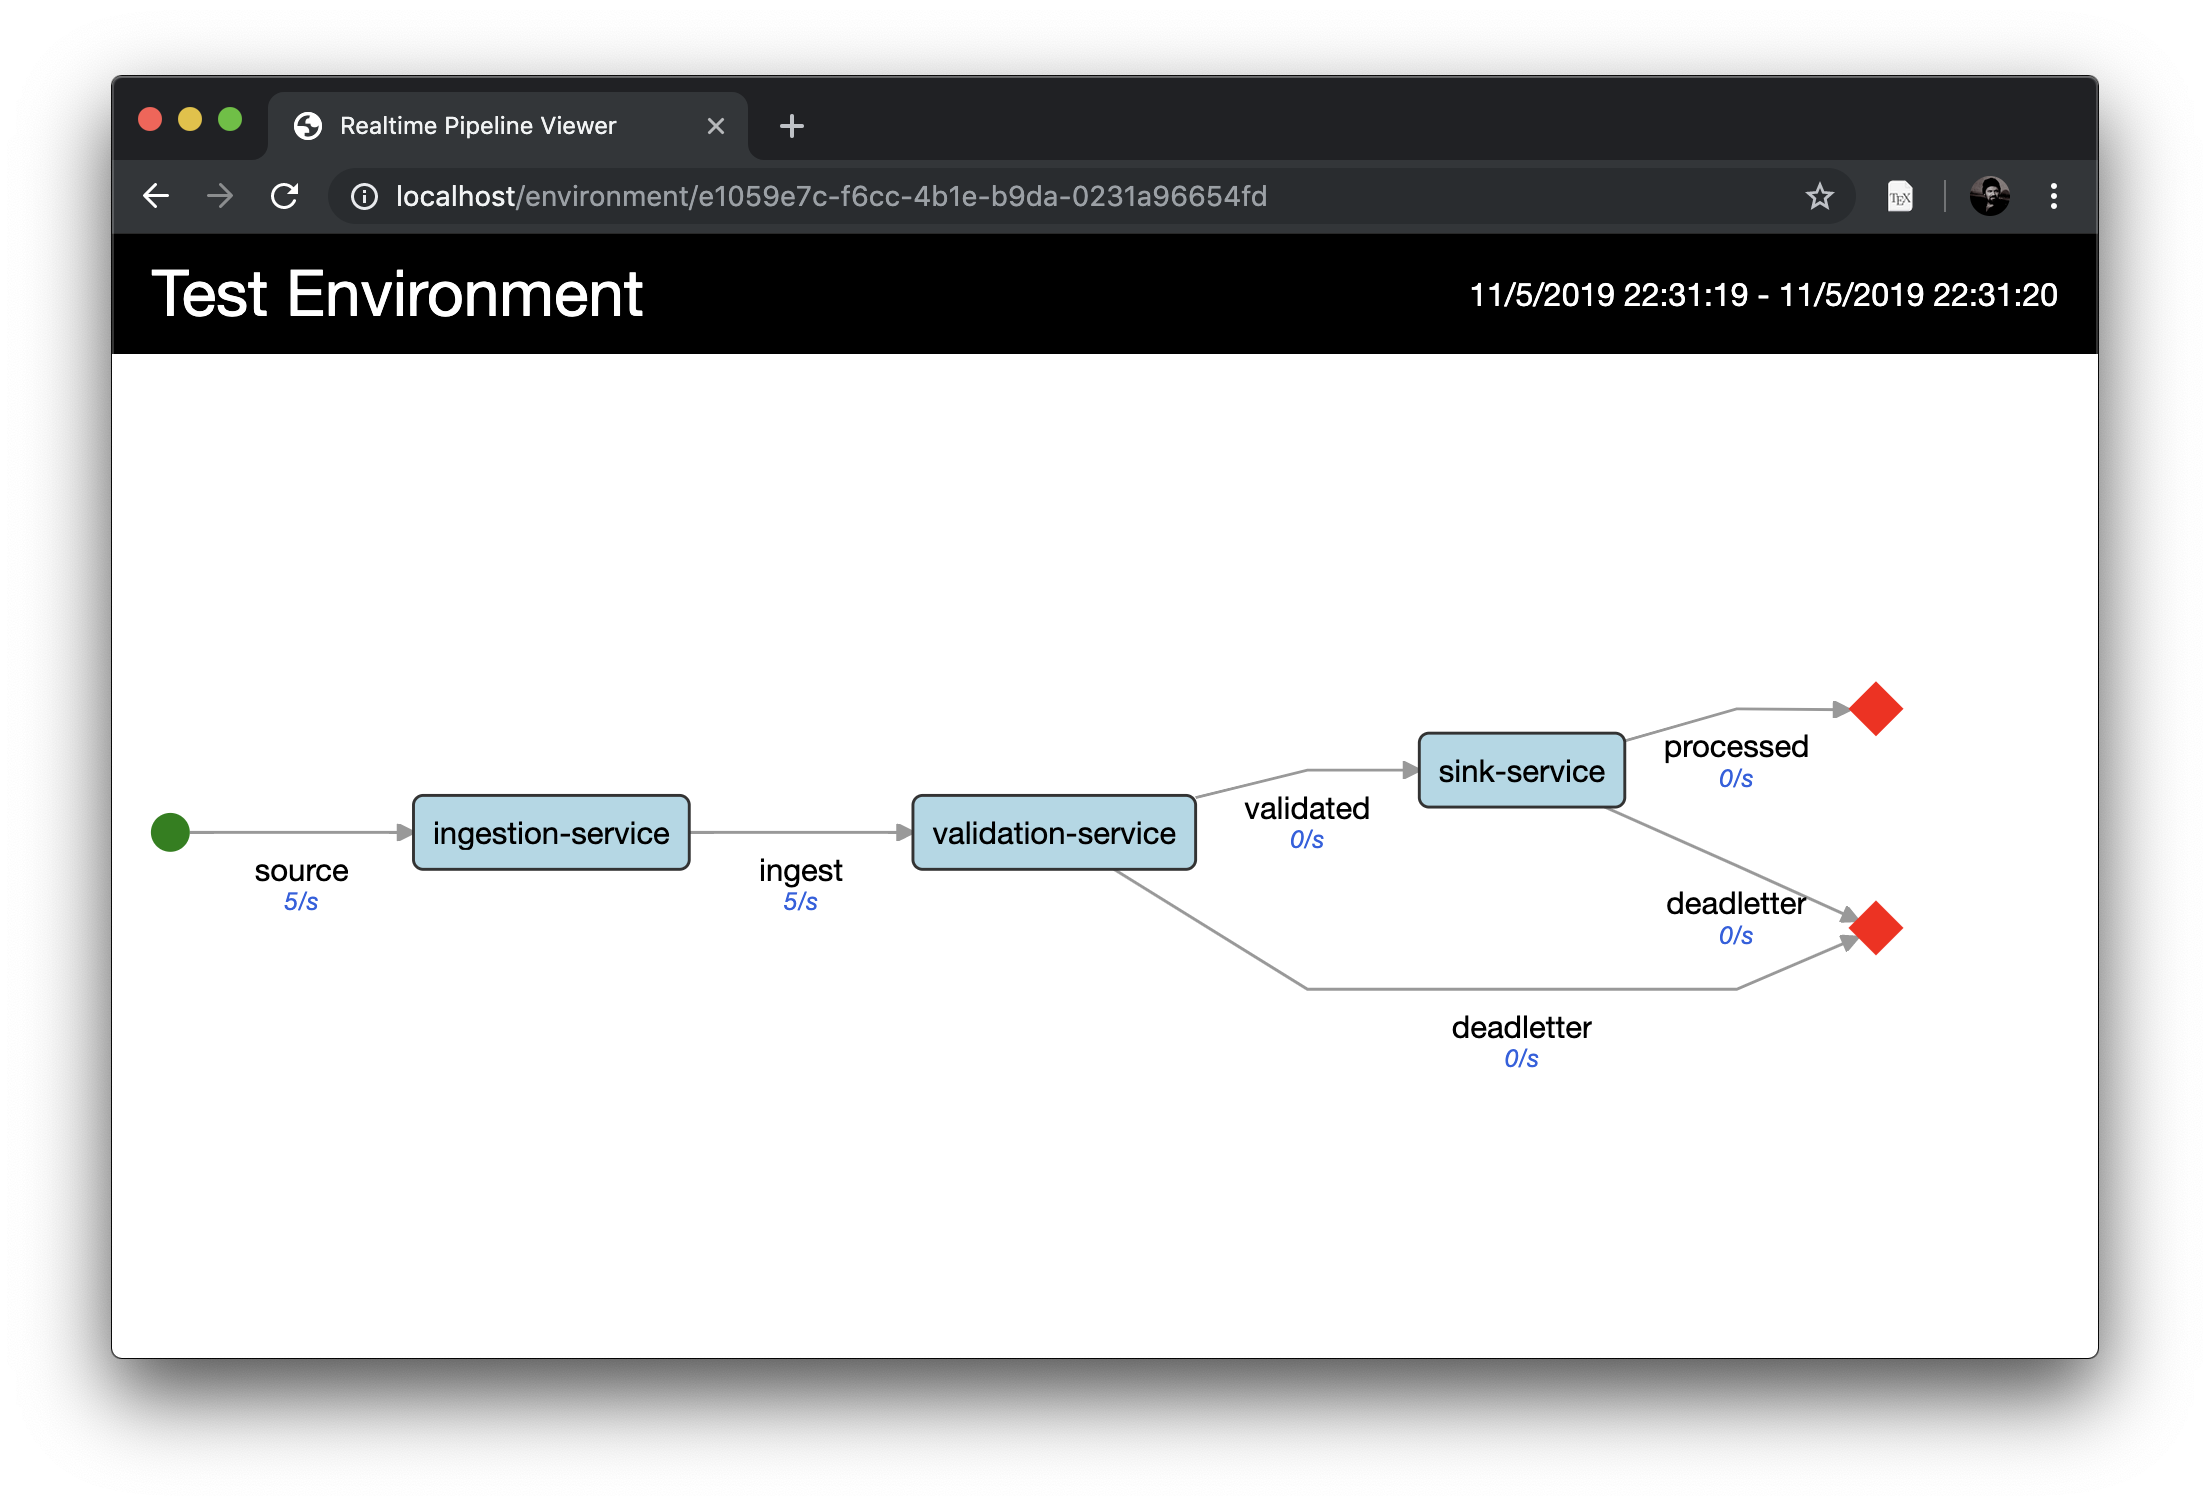
\includegraphics[scale=0.4]{figures/walkthrough/correlation_env_activity.png}
	\caption{Dashboard Client - message activity in an environment discovered by message correlation.}
	\label{activity_env_correlation}
\end{figure}


\end{enumerate}